\documentclass[12pt, a4paper]{report}

% --- Impostazioni di stile ---
\usepackage{document_style}

% --- Tikz externalize
\usetikzlibrary{external}
\tikzexternalize[prefix=build_tikzexternal/]

% ------------------------------------------------------------------------------------
%                               INIZIO DOCUMENTO
% ------------------------------------------------------------------------------------

\begin{document}
\pagestyle{fancy}

% --- Inizio documento ---
\begin{titlepage}
    \centering
    
    % --- INTESTAZIONE AUTORI ---
    \vspace*{2cm}
    {\large \textsc{Davide Pozzebon}}\\[3cm]
    
    % --- TITOLO PRINCIPALE ---
    {\Huge \textsc{Modelli e Software per}}\\[0.3cm]
    {\Huge \textbf{\textit{\textcolor{nord11}{L'OTTIMIZZAZIONE DISCRETA}}}}\\[1.5cm]
    
    % --- SOTTOTITOLO ---
    {\Large \textsc{Appunti del Corso}}\\[2cm]
    
    \vfill
    
    % --- INFO ANNO ACCADEMICO ---
    {\large \textsc{Ingegneria Informatica -- UniPD}}\\[0.3cm]
    {\large Anno Accademico 2026--2027}
    
    \vspace*{1cm}
\end{titlepage}

\thispagestyle{empty} % Rimuove il numero di pagina da questa pagina

% --- PARTE SUPERIORE CENTRATA ---
\vspace*{5cm}
\begin{center}
    {\large Davide Pozzebon}\\[0.5cm]
    {\itshape Modelli e Software per l'Ottimizzazione Discreta -- Appunti}\\[0.5cm]
\end{center}

\vspace*{\fill}

% --- PARTE INFERIORE SINISTRA ---
\noindent \textbf{\textsc{Descrizione dei contenuti}}

\vspace{0.5em}
\noindent \small
Questo lavoro è un resoconto dettagliato del corso di 
\textit{Modelli e Software per l'Ottimizzazione Discreta} della laurea 
triennale in Ingegneria Informatica presso l'Università degli Studi di Padova.

\vspace{1.5em}
\noindent \textbf{\textsc{Sorgente e altri appunti}}

\vspace{0.5em}
\noindent \small
Il documento originale è reperibile, insieme anche agli appunti di altri corsi del
curriculum della laurea, dalla repository GitHub al link seguente:
\href{https://github.com/DavidePoz/Ingegneria-Informatica---Appunti.git}
     {github.com/DavidePoz/Ingegneria-Informatica---Appunti}

\vspace*{1cm}


% Indice
\tableofcontents

% --- Capitoli principali ---
% ------------------------------------------------------------------------------------
%                               NOZIONI INTRODUTTIVE
% ------------------------------------------------------------------------------------

\chapter{Nozioni introduttive}

\begin{definition}[OTTIMIZZAZIONE MATEMATICA]
    L'\textbf{ottimizzazione} (o programmazione matematica, PM) è una branca della 
    matematica applicata che studia \textbf{teoria e metodi} per la \textbf{ricerca 
    dei punti di massimo e minimo di una funzione} all'interno di un dominio specificato.
\end{definition}

Per cui, per poter applicare l'ottimizzazione matematica abbiamo bisogno di:
\begin{enumerate}
    \item Un \textbf{insieme di decisioni} (che costituiranno la funzione da ottimizzare).
    \item Poter \textbf{misurare il risultato delle decisioni}.
    \item Poter \textbf{confrontare la "bontà" delle decisioni}.
\end{enumerate}

\section{Modellare la realtà}

In generale, l'ottimizzazione matematica è utilizzata per \textbf{trovare soluzioni ottimali}
a \textbf{problemi reali} (in ambito ingegneristico, industriale, economico-finanziario etc.).

Per prima cosa, abbiamo quindi bisogno di \textbf{creare un modello} che \textbf{descriva
il problema reale}; poi procederemo a \textbf{risolverlo} e, infine, dovremmo
\textbf{interpretare la soluzione} trovata:

\begin{figure}[!ht]
    \centering
    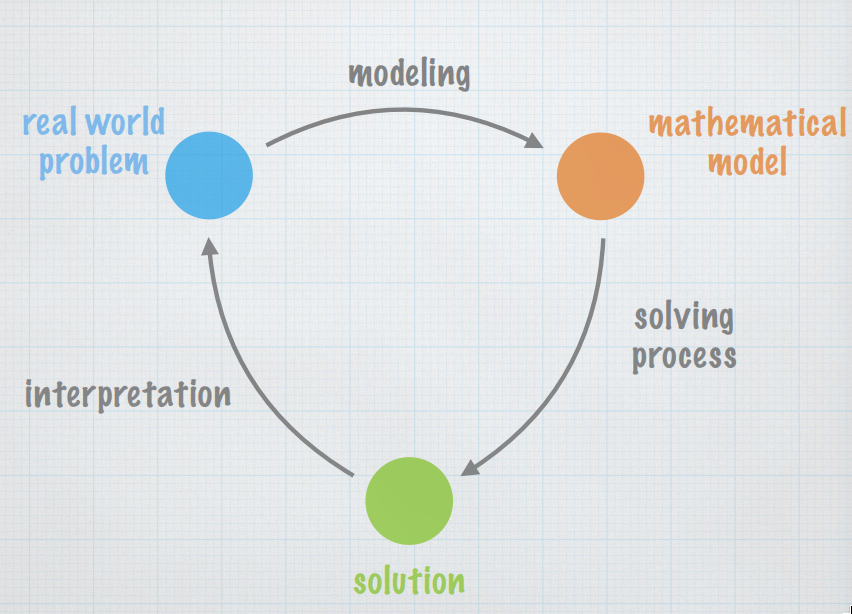
\includegraphics[scale=0.2]{images/01_00_SchemaApplicazioneOttimizzazione.png}
    \caption{Schema di applicazione dell'ottimizzazione matematica}
\end{figure}

\begin{warn}
    La fase di \textbf{interpretazione} è \textbf{spesso sottovalutata}: è
    \textbf{importantissimo} interpretare i risultati per capire
    \textit{cosa rappresentano} e, soprattutto, se \textit{sono compatibili
    con la realtà}.
\end{warn}

\section{Modelli matematici e ottimizzazione}

In generale, i modelli matematici sono delle formulazioni del problema $P$ del tipo:

\begin{definition}[FORMULAZIONE PROBLEMA DI OTTIMIZZAZIONE]
    \[
        \begin{aligned}
            \text{min/max }f(x)& \\ 
            S& \\ 
            x\in D&
        \end{aligned}
    \]
    Dove $f(x)$ è la \textbf{funzione obiettivo} nelle variabili reali $x=(x_{1},\ldots,x_n)$,
    $D=D_{1}\times \ldots \times D_n$ è il dominio di $x$, ed $S$ è un 
    \textbf{insieme finito di vincoli}.
\end{definition}

In genere si considerano problemi di ottimizzazione in cui vogliamo minimizzare la funzione
obiettivo, ma possiamo "convertire" un modello in una o nell'altra forma a piacimento.
Chiariamo ora alcuni dettagli:

\begin{definition}[OTTIMIZZAZIONE DISCRETA]
    Se il dominio $D$ è \textbf{discreto}, si parla di \textbf{ottimizzazione discreta}.
\end{definition}

\begin{definition}[OTTIMIZZAZIONE COMBINATORIA]
    Se il dominio $D$ è \textbf{discreto e finito}, allora si parla di
    \textbf{ottimizzazione combinatoria}.
\end{definition}

\begin{definition}[SOLUZIONE]
    Ogni $x\in D$ è \textbf{soluzione} del problema $P$.
\end{definition}

\begin{definition}[VINCOLO]
    Un vincolo $c\in S$ è una \textbf{funzione} associata ad un
    \textbf{sottoinsieme di variabili} $x_c$, il cui valore può essere
    \textbf{vero} (in tal caso il vincolo è \textbf{soddisfatto}), oppure
    \textbf{falso} (in tal caso il vincolo è \textbf{violato}).
\end{definition}

\begin{definition}[SOLUZIONE AMMISSIBILE]
    Una \textbf{soluzione} che \textbf{rispetti tutti i vincoli} si 
    dice \textbf{ammissibile}.

    L'\textbf{insieme} delle soluzioni ammissibili si indica con $F(P)$.
\end{definition}

\begin{definition}[SOLUZIONE OTTIMA]
    Una soluzione ammissibile $x^*$ si dice \textbf{ottima} se
    \[
        f(x^*) \le f(x) \text{ , } \forall x \in F(P)
    \] 
\end{definition}

Inoltre:

\begin{definition}[PROBLEMA IMPOSSIBILE]
    Un problema di ottimizzazione si dice \textbf{impossibile} (\textit{infeasible})
    se \textbf{non ammette alcuna soluzione ammissibile}, cioè
    $F(P) = \emptyset$
\end{definition}

\begin{definition}[PROBLEMA ILLIMITATO]
    Un problema di ottimizzazione si dice \textbf{illimitato} (\textit{unbounded}) 
    se \textbf{non esiste} alcun \textbf{limite inferiore} a $f(x)$ per $x\in F(P)$.
\end{definition}

\begin{definition}[PROBLEMA RISOLTO]
    Un problema di ottimizzazione si dice \textbf{risolto} quando ne viene
    \textbf{trovata una soluzione ottima} (dimostrando che è tale), oppure 
    quando si \textbf{dimostra che il problema è impossibile o illimitato}.
\end{definition}

E' inoltre importante chiarire il seguente dettaglio:

\begin{warn}[MODELLAZIONE VS RISOLUZIONE]
    In questo corso ci concentreremo sulla fase di \textbf{modellizzazione}.
    Questo perchè:
    \begin{itemize}
        \item Gli \textit{algoritmi risolutivi} sono \textit{incredibilmente 
            complessi} e sono diventati 4-5 ordini di grandezza più
            efficienti nel corso degli ultimi 50 anni; studiarli da zero
            rappresenterebbe solo un handicap.
        \item La fase di modellizzazione è comunque molto importante
            come strumento a disposizione di un ingegnere.
    \end{itemize}
\end{warn}

\section{Paradigmi di ottimizzazione}

Purtroppo, un problema di ottimizzazione \textbf{arbitrario} è \textbf{indecidibile}: è
quindi necessario aggiungere dei vincoli alla \textit{"forma del problema"}.

Chiaramente, imporre dei vincoli ai modelli significa anche \textbf{ridurne l'espressività}
(ovvero possiamo rappresentare fedelmente meno problemi reali); tuttavia esistono due
paradigmi di ottimizzazione che rappresentano un \textbf{buon compromesso} tra \textit{espressività}
e \textit{risolubilità}:
\begin{enumerate}
    \item \textbf{Programmazione Lineare}(PL) - trattata nel corso.
    \item \textbf{Ottimizzazione Convessa} - non trattata nel corso.
\end{enumerate}

\begin{remark}[PROGRAMMAZIONE LINEARE]
    Nella programmazione lineare, la \textbf{funzione obiettivo} ed i \textbf{vincoli}
    sono \textbf{lineari} (duh!). 

    Per quanto stringente possa sembrare questa limitazione,
    moltissimi problemi possono essere modellati in questo modo e, inoltre, si
    tratta di una branca assai matura.
\end{remark}

Di seguito vediamo più nel dettaglio alcuni paradigmi di nostro interesse.

\subsection{Programmazione Lineare}

Un problema di \textbf{programmazione lineare} (LP) consiste nella minimizzazione di 
una \textbf{funzione lineare} soggetta ad un numero finito di \textbf{vincoli lineari}. 
In generale si ha la forma:

\begin{definition}[PROBLEMA DI PROGRAMMAZIONE LINEARE]
    \[
        \begin{aligned}
            \text{min } &c^\top x \\ 
                        &a_i^\top x \sim b_i \text{ , }i=1,\ldots,m \\ 
                        &l_j \le x_j \le u_j \text{ , }j=1,\ldots ,n
        \end{aligned}
    \] 
    Con $\sim \in \{\le , =, \ge \}  $, $l_j\in \mathbb{R} \cup \{-\infty\}  $ 
    e $u_j\in \mathbb{R}\cup \{+\infty\}$.
\end{definition}

Chiariamo ora alcuni dettagli sulle variabili nella definizione:

\begin{remark}[RUOLO DELLE VARIABILI NELLA DEFINIZIONE]
    Le variabili nella definizione hanno i seguenti ruoli:
    \begin{itemize}
        \item Le variabili $x_{1},\ldots,x_n$ compongono il \textbf{vettore delle decisioni} $x$.
        \item $c\in \mathbb{R}^n$ \textit{pesa le variabili} di nostro interesse per
            ottenere la \textit{funzione obiettivo} $c^\top x$.
        \item I vettori $a_i^\top\in \mathbb{R}^n$ \textit{pesano ogni variabile} per
            formalizzare i \textit{vincoli} $i=1,\ldots ,m$.
        \item Il vettore $b=(b_{1},\ldots ,b_m)\in \mathbb{R}^m$ completa la 
            formalizzazione dei vincoli.
    \end{itemize}
\end{remark}

\subsection{Programmazione Lineare Intera}

Un problema di \textbf{programmazione lineare intera}(Mixed Integer Programming) 
consiste nella minimizzazione diuna funzione lineare soggetta ad un numero 
finito di vincoli lineari, con in più il vincolo che \textbf{alcune variabili} 
devono assumere \textbf{valori interi}.

\begin{definition}[PROBLEMA MIP]
    \[
        \begin{aligned}
            \text{min } &c^\top x \\ 
                        &a_i^\top x \sim b_i \text{ , }i=1,\ldots,m \\ 
                        &l_j \le x_j \le u_j \text{ , }j=1,\ldots ,n \\ 
                        &x_j \in \mathbb{Z} \text{ , } \forall j\in J \subseteq N = \{1,\ldots ,n\}  
        \end{aligned}
    \] 
    Con $\sim \in \{\le , =, \ge \}  $, $l_j\in \mathbb{R} \cup \{-\infty\}  $ 
    e $u_j\in \mathbb{R}\cup \{+\infty\}$ come prima.
\end{definition}

Da notare che se $J=N$ si parla di \textit{programmazione lineare intera} \textbf{pura} 
(\textbf{tutte} le variabili sono \textbf{intere}), mentre se $J=\emptyset$ si
ha a che fare con un problema di programmazione lineare classica.

\subsection{Programmazione con Vincoli}

Un problema di \textbf{programmazione con vincoli} è definito da una \textbf{terna} 
$(X, D, C)$, dove $X$ è un insieme di variabili con \textbf{dominio finito} $D$, 
e $C$ è un insieme finito di \textbf{vincoli di natura arbitraria}.

\begin{remark}
    Il paradigma CP è \textbf{molto più libero} nella definizione dei vincoli 
    che si possono usare per modellare un problema. 
    Questo fa si che spesso la modellazione sia più immediata e compatta.

    Di contro, se i vincoli usati \textbf{non} hanno una \textbf{struttura} che 
    \textbf{permetta lo sviluppo di algoritmi efficienti}, la \textbf{capacità di 
    risoluzione} sarà al contrario \textbf{penalizzata}.
\end{remark}

\subsection{Soddisfacibilità booleana}

Un problema di \textbf{soddisfacibilità booleana} è un caso particolare di problema
di \textit{soddisfacibilità}.

\begin{definition}[PROBLEMA DI SODDISFACIBILITA' BOOLEANA]
    \textbf{Tutte le variabili} sono \textbf{booleane} (cioè possono assumere solo i 
    valori \textit{True} o \textit{False} e i \textbf{vincoli} sono un numero 
    finito di \textbf{clausole booleane}.
\end{definition}

Come nel caso LP/MIP, in un problema SAT il \textbf{linguaggio a disposizione} per modellare un
problema di ottimizzazione viene \textbf{notevolmente ristretto}.

\begin{remark}
    Nonostante ciò, molti problemi di notevole importanza pratica, come la 
    \textbf{progettazione di circuiti logici}, possono essere espressi naturalmente 
    con questo paradigma.
\end{remark}

% ------------------------------------------------------------------------------------
%                                CONCETTI GENERALI
% ------------------------------------------------------------------------------------

\chapter{Concetti generali dell'ottimizzazione}

\section{Nozioni paradigma-indipendenti}

La teoria e gli algoritmi sviluppati per affrontare problemi nei quattro paradigmi presentati
sopra sono notevolemente diversi gli uni dagli altri; tuttavia esistono \textbf{alcuni concetti 
fondamentali} che sono \textbf{comuni a tutti gli approcci dell'ottimizzazione}, anche 
\textbf{indipendentemente dal paradigma}. 

\subsection{Inferenza}

In un problema di ottimizzazione, può capitare che un \textbf{vincolo} $C$ sia
\textbf{dedotto} (derivato) da un \textbf{insieme di vincoli} $S$.

\begin{definition}[VINCOLO DEDOTTO]
    Se \textbf{ogni} $x\in D$ che \textbf{soddisfa} $S$ \textbf{soddisfa
    anche} $C$, allora diciamo che $C$ è un \textbf{vincolo dedotto}.
\end{definition}

Chiaramente, dal punto di vista della modellazione, un tale vincolo è \textbf{ridondante}
dato che \textbf{non cambia l'insieme delle soluzioni ammissibili}; tuttavia potrebbe
rivelarsi (in alcuni casi) molto utile per \textbf{l'efficienza degli algoritmi di 
ricerca} in quanto potrebbe \textit{"esplicitare" informazioni} che \textit{non sono
derivabili da nessun altro vincolo se preso singolarmente}.

\begin{exa}
    Consideriamo ad esempio la seguente regione ammissibile:
    \[
        \begin{aligned}
            x_{1} + x_{2} \ge 1 & & x_{1}-x_{2} \ge 0 & & x_{1},x_{2} \in \{0,1\}  
        \end{aligned}
    \]
    E' immediato verificare che $x_{1}=1$ è un \textbf{vincolo valido} per $S$, ma
    \textbf{non è immediatamente deducibile} dai due vincoli sopra se 
    \textbf{presi separatamente}.
\end{exa}

\subsection{Ricerca}

Un concetto molto importante è quello di ricerca:

\begin{definition}[RICERCA]
    Dato un problema $P$, la \textbf{ricerca} consiste nel \textbf{risolvere una serie di
    restrizioni} 
    \[
        P_{1}, \ldots , P_m 
    \] 
    di $P$.

    Le \textbf{restrizioni} sono \textbf{ottenute aggiungendo dei vincoli} al
    problema originale.
\end{definition}

In altre parole, rendiamo \textit{più "stringente"} il problema andando ad aggiungere
ulteriori vincoli. L'intuizione alla base delle restrizioni è che in alcuni casi
potrebbe risultare \textit{conveniente} aggiungere dei vincoli per \textbf{restringere 
lo spazio delle soluzioni}, in modo tale da rendere il problema \textbf{più
facile da risolvere}.

In particolare, sono importanti le \textbf{ricerche esaustive}:

\begin{definition}[RICERCA ESAUSTIVA]
    Una ricerca si dice \textbf{esaustiva} se l'insieme delle restrizioni considerate
    \textbf{"copre" tutto lo spazio} delle \textbf{soluzioni ammissibili} di $P$:
    \[
        \bigcup_i F(P_i) = F(P)
    \] 
\end{definition}

Nel caso di una ricerca esaustiva, possiamo \textbf{rivolvere} $P$ \textbf{risolvendo
tutte le restrizioni} $P_i$ e \textbf{scegliendo la soluzione migliore}.

In ogni caso, è importante il seguente fatto:

\begin{prop}
    Data una restrizione $P_i$, una \textbf{sua qualsiasi soluzione
    ammissibile} è \textbf{ammissibile anche} per il problema di partenza $P$.

    In particolare se $\tilde{x}$ è \textbf{soluzione ottima della restrizione}, essa
    rappresenta un \textbf{upper bound} per la \textbf{soluzione al problema 
    originale} $x^{*}$:
    \[
        x^* \le \tilde{x}
    \] 
\end{prop}

L'intuizione dietro al fatto è la seguente:

\begin{remark}[INTUIZIONE]
    Le soluzioni di $P_i$ sono un \textbf{sottoinsieme delle soluzioni originali},
    per cui una soluzione di $P_i$ deve \textbf{essere anche soluzione} di $P$.

    Inoltre, se $\tilde{x}$ è \textbf{soluzione ottima della restrizione}, sappiamo
    che la \textbf{soluzione al problema originale} sarà \textbf{"almeno così
    tanto buona"}.
\end{remark}

\subsection{Rilassamento}

Il \textit{rilassamento} è il concetto complementare alla restrizione. Un 
rilassamento $R$ è ottenuto da un problema di ottimizzazione $P$:
\begin{enumerate}
    \item Eliminando alcuni vincoli.
    \item Sostituendo la funzione obiettivo $f(x)$ con la sua \textit{approssimazione
        inferiore} $g(x)$.
\end{enumerate}

Più formalmente:

\begin{definition}[RILASSAMENTO]
    $R$ è un \textbf{rilassamento} di $P$ se:
    \begin{enumerate}
        \item $F(P) \subseteq F(R)$
        \item $g(x)\le f(x)$  $\forall x\in F(P)$
    \end{enumerate}
\end{definition}

In maniera analoga a quanto detto per le restrizioni, l'idea è che a volte 
potrebbe risultare più semplice risolvere una \textit{"versione rilassata"} del
problema.

\begin{warn}
    Sebbene si possano ricavare informazioni utili, bisogna fare attenzione 
    al fatto che il \textbf{problema NON è equivalente}.
\end{warn}

In tal senso, è utile considerare le seguenti proposizioni:

\begin{prop}
    Dato un problema $P$ ed un suo rilassamento $R$ è possibile derivare che:
    \begin{enumerate}
        \item Se $F(R)=\emptyset$, allora $P$ è \textbf{impossibile}.
        \item Se $x^*$ è \textbf{soluzione ottima} di $R$, $g(x^*)$ è un \textbf{lower
            bound} per il \textbf{valore ottimo} di $P$.
        \item Se $x^*$ è \textbf{soluzione ottima} di $R$, $x^*\in F(P)$ e
            $g(x^*)=f(x^*)$, allora $x^*$ è \textbf{ottima} per $P$.
    \end{enumerate}
\end{prop}

E' utile discutere i tre punti:

\begin{remark} Possiamo intuire che:
    \begin{enumerate}
        \item Se il \textbf{rilassamento} (la versione "semplificata") 
            è \textbf{impossibile}, lo \textbf{deve essere anche
            il problema originale}.
        \item La soluzione ottima del rilassamento ci fornisce un
            \textbf{"tetto massimo"} per la \textbf{"bontà" della soluzione}: avendo
            "accesso" solo ad un sottoinsieme delle soluzioni, quella di nostro
            interesse sicuramente \textit{non potrà essere migliore}.
        \item Si tratta di un \textbf{caso fortunato}: se la soluzione del rilassamento
            è \textbf{ottima}, \textbf{ammisibile} per $P$, e i \textbf{valori delle
            funzioni obiettivo coincidono}, allora $x^*$ è \textbf{ottima anche per} $P$.
    \end{enumerate}
\end{remark}

\subsection{Dualità}

Un problema di ottimizzazione $P$ viene spesso \textbf{interpretato come problema di 
ricerca} (problema \textit{primario}): vogliamo \textbf{"cercare" la soluzione ottima}.

Alternativamente, lo stesso problema può anche essere visto come un \textbf{problema
di inferenza} (problema \textit{duale}): a partire dai vincoli, vogliamo \textbf{derivare il più stretto
lower bound possibile} su $f(x)$.

\begin{definition}[PROBLEMA DUALE]
    Il problema di \textbf{trovare la dimostrazione} che \textbf{porta al
    lower bound più stretto} prende il nome di \textbf{problema duale}.
\end{definition}

\begin{remark}[INTERPRETAZIONE]
    In altre parole:
    \begin{itemize}
        \item Il problema \textbf{originale} cerca di \textbf{"scendere" verso il valore minimo} 
        trovando \textbf{soluzioni ammissibili via via migliori}, 
        \item Il problema \textbf{duale} cerca di \textbf{"salire"} costruendo un 
        \textbf{limite inferiore sempre più alto}, manipolando i vincoli a disposizione. 
    \end{itemize}
\end{remark}

Questo è un punto cardine della programmazione matematica, dato che permette di 
\textbf{certificare l'ottimalità di una soluzione}: quando il \textbf{valore ottenuto dalla ricerca} 
coincide con il \textbf{limite inferiore dimostrato dall'inferenza}, si ha la \textbf{garanzia} di aver 
trovato l'\textbf{ottimo globale}.

\section{Approcci di ricerca}

\subsection{Ricerca naive: Generate-And-Test}

Un possibile approccio per applicare la ricerca ad un problema di ottimizzazione
è \textit{generate-and-test}. Banalmente, l'idea di base è la seguente:

\begin{definition}[GENERATE-AND-TEST]
    Generiamo \textbf{tutte le soluzioni} possibili, poi le \textbf{confrontiamo}
    e \textbf{scegliamo la migliore}.
\end{definition}

Formalmente, si tratta di considerare \textbf{tutte le restrizioni} in cui
$x$ è \textbf{fissato} (cioè tutti i suoi possibili valori); è quindi chiaro
che questo approccio è applicabile solo in caso di problemi di \textbf{ottimizzazione
combinatoria}, in cui il \textit{numero di soluzioni è finito}.

E' importante notare che:

\begin{warn}
    La complessità computazionale di questo approccio è \textbf{sempre} 
    $O(\beta^n)$, dove $\beta$ è il numero di valori che possono
    assumere le variabili $x_i$.
\end{warn}

Ciò non significa che non sia mai applicabile, vuol semplicemente dire che
i suoi casi applicativi sono piuttosto \textit{rari/particolari}. Se per esempio
il problema coinvolgesse \textit{poche variabili}, ma con \textit{vincoli non lineari
particolarmente complessi}, \textit{"testare" tutte le soluzioni} potrebbe 
risultare \textit{più conveniente che "risolvere i vincoli"}.

\subsection{Ricerca ad albero: Branch-and-Bound}

Un'approccio \textit{"più strutturato"} è quello della \textbf{ricerca ad albero}.
L'idea di base è la seguente:

\begin{definition}[RICERCA AD ALBERO]
    Vogliamo \textbf{partizionare} lo spazio delle \textbf{soluzioni possibili},
    \textbf{iterando ricorsivamente} il metodo fino a quando otteniamo
    \textbf{partizioni sufficientemente facili da risolvere}.
\end{definition}

L'idea è che \textit{dopo una serie di iterazioni}, il problema sarà stato
\textit{scomposto abbastanza} da essere diventato \textit{più facile da risolvere},
per una qualche definizione di "più facile da risolvere". E' tuttavia 
importante notare che:

\begin{warn}
    Al \textbf{caso peggiore}, questo algoritmo è \textbf{peggio di generate-and-test}.
    Si tratta del caso in cui \textit{generiamo tutte le soluzioni} (come generate-and-test): in
    questo caso, avremmo anche l'\textit{aggiunta di tutti i passaggi intermedi} (per ottenere
    le restrizioni).
\end{warn}

Un'esempio di ricerca ad albero è data dall'algoritmo \textit{Branch-and-Bound}, che
usa una strategia \textbf{divide and conquer} per trovare la soluzione ottimale.
In particolare, costruisce un \textbf{albero di restrizioni}, sulle quali \textbf{risolve
dei rilassamenti} per determinare se è possibile eliminare dei rami.

\begin{definition}[BRANCH-AND-BOUND]
    Sia $P$ un problema di ottimizzazione con funzione obiettivo $f(x)=c^\top x$ 
    (da \textbf{minimizzare}), sia $\overline{x}\in F(P)$, e sia
    $z=f(\overline{x})$ un \textbf{upper bound} (iniziale) per il problema,
    detto \textbf{incumbent}.

    Sia $A$ una \textbf{coda} di problemi inizializzata con $P$: $A=[P]$.
    \textbf{Finchè $A$ non è vuota, si ripetono} le seguenti operazioni:
    \begin{enumerate}
        \item Si \textbf{sceglie un problema} $P_i$ di $A$
        \item Si \textbf{risolve un rilassamento}$R_i$ di $P_i$, e:
            \begin{enumerate}
                \item Se \textbf{non ammette soluzione}, si può 
                    \textbf{eliminare il ramo}
                \item Se la \textbf{soluzione del rilassamento} è \textbf{maggiore}
                    dell'\textbf{incumbent}, si può \textbf{eliminare il ramo}.
                \item Se la \textbf{soluzione} del rilassamento è 
                    \textbf{ammissibile} per il problema originale $P$ ed
                    è \textbf{minore} dell'\textbf{incumbement}, \textbf{aggiorniamo
                    quest'ultimo} con il nuovo valore trovato.
            \end{enumerate}
        \item Se il problema \textbf{non è stato scartato}, allora si \textbf{restringe
            ulteriormente}: $F(P_i)=\bigcup_j F(P_{ij})$.
        \item Si \textbf{rimuove il problema} $P_i$ (lasciando solo le sue restrizioni).
    \end{enumerate}
\end{definition}

Vale la pena discutere le decisioni prese al punto due:

\begin{remark}
    Le scelte prese al punto due derivano dai seguenti fatti:
    \begin{enumerate}
        \item Se il \textit{rilassamento della restrizione considerata} è \textit{impossibile}
            possiamo scartare quel \textit{branch} perchè \textit{sappiamo già} che 
            anche \textit{tutte le successive restrizioni sarebbero impossibili}.
        \item Similmente, se la soluzione è \textit{peggiore dell'incumbent} attuale,
            sappiamo già che \textit{anche tutte le soluzioni delle successive
            restrizioni lo saranno}.
        \item Se la soluzione trovata è \textit{migliore di quella attualmente 
            conosciuta}, allora essa diventa la nostra \textit{nuova miglior stima} 
            e possiamo \textit{aggiornare l'incumbent}.
    \end{enumerate}
\end{remark}

\begin{figure}[!ht]
    \centering
    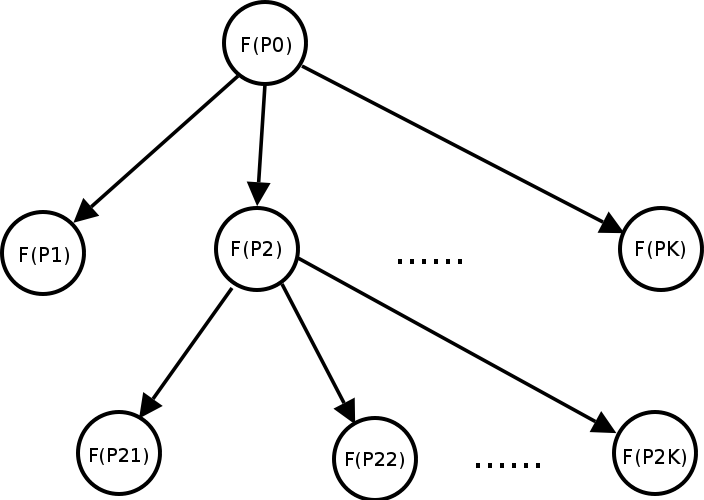
\includegraphics[scale=0.7]{images/02_00_Branch_and_Bound.png}
    \caption{Esempio di albero associato all'esecuzione dell'algoritmo}
\end{figure}

E' inoltre importante tenere a mente che:

\begin{remark}[EFFICIENZA DELL'ALGORITMO]
    L'efficienza dell'algoritmo è \textbf{fortemente influenzata} da:
    \begin{enumerate}
        \item \textbf{Partizionamento del problema} nelle sue restrizioni.
        \item \textbf{Scelta dei rilassamenti} associati alle restrizioni (bisogna
            generare \textit{problemi semplici da risolvere}, ma che contrinuiscano
            con \textit{lower bound ragionevoli}).
    \end{enumerate}
\end{remark}

Infine, ricollegandoci a quanto detto sopra sugli algoritmi di ricerca ad albero al
caso peggiore, sottolineaiamo che:

\begin{remark}
    Branch and Bound è un \textit{algoritmo di enumerazione implicita} perché si comporta 
    esattamente come un \textit{algoritmo di enumerazione} (cioè "prova" tutte le soluzioni 
    possibili fino a trovare quella ottima), ma ne \textbf{scarta alcune} dimostrando 
    a priori la loro \textit{non ottimalità}.
\end{remark}

% ------------------------------------------------------------------------------------
%                           PROGRAMMAZIONE LINEARE - IN DEPTH
% ------------------------------------------------------------------------------------

\chapter{Programmazione Lineare}

Torniamo ora al paradigma della \textbf{programmazione lineare} per
discuterlo più nel dettaglio.

\section{Forma standard e forma canonica}

Abbiamo già visto una possibile forma in cui può presentarsi un problema
di programmazione lineare nel capitolo introduttivo.

Ora, senza perdita di generalità, possiamo assumere che il problema sia espresso 
in \textbf{forma standard}: 

\begin{definition}[FORMA STANDARD]
    \[
        \begin{cases}
            \text{min } c^\top x \\ 
            Ax = b \\ 
            x_i \ge 0
        \end{cases}
    \] 
\end{definition}

Oppure in \textbf{forma canonica}:

\begin{definition}[FORMA CANONICA]
    \[
        \begin{cases}
            \text{min } c^\top x \\ 
            Ax \ge  b \\ 
            x_i \ge 0
        \end{cases}
    \] 
\end{definition}

\begin{remark}
    Il nome di queste forme deriva dal fatto che \textbf{qualsiasi altro problema 
    di programmazione lineare} è \textbf{riconducibile a queste}.
\end{remark}

\subsection{Formulazioni equivalenti}

Possiamo \textbf{passare} da una \textbf{formulazione generica} di un problema
di programmazione lineare ad una \textbf{forma standard (o canonica) equivalente} applicando
le regole di trasformazione seguenti:

\begin{enumerate}
    \item Conversione da \textbf{massimizzazione a minimizzazione}
        \[
            \text{max}(c^\top x) = -\text{min}(-c^\top x)
        \] 
    \item Conversione da \textbf{vincoli} "$\ge $" a vincoli "$=$"
        \[
            a_i^\top x \ge b_i \Longleftrightarrow \begin{cases}
                a_i^\top x - s_i = b_i \implies a_i^\top x = b_i'  \\ 
                s_i \ge 0
            \end{cases}
        \] 
    \item Conversione da \textbf{vincoli} "$\le $" a vincoli "$=$"
        \[
            a_i^\top x \le b_i \Longleftrightarrow \begin{cases}
                a_i^\top x + s_i = b_i \implies a_i^\top x = b_i'  \\ 
                s_i \ge 0
            \end{cases}
        \]
    \item Conversione da \textbf{vincoli} "$=$" a vincoli "$\ge$"
        \[
            a_i^\top x = b_i \Longleftrightarrow \begin{cases}
                a_i^\top x \ge  b_i  \\ 
                -a_i^\top x \ge -b_i
            \end{cases}
        \] 
    \item Conversione da \textbf{variabili libere} a \textbf{non negative}
        \[
            x_i \text{ libera } \Longleftrightarrow \begin{cases}
                x_i = x_i^+ - x_i^- \\ 
                x_i^+,x_i^- \ge 0
            \end{cases}
        \] 
    \item Conversione da \textbf{lower bound generico} a \textbf{variabile non negativa}
        \[
            x_i \ge l_i \Longleftrightarrow \begin{cases}
                x_i = x_i' + l_i \\
                x_i' \ge0
            \end{cases}
        \] 
    \item Conversione da \textbf{upper bound generico} a \textbf{variabile non negativa}
        \[
            x_i \le u_i \Longleftrightarrow \begin{cases}
                x_i = u_i - x_i' \\
                x_i' \ge0
            \end{cases}
        \]
    \item Conversione da \textbf{variabile bounded} a \textbf{variabili non negative}
        \[
            l_i \le  x_i \le u_i \Longleftrightarrow \begin{cases}
                x_i = x_i' + l_i \\
                x_i' + s_i = u_i - l_i \\
                x_i', s_i \ge0
            \end{cases}
        \] 
\end{enumerate}

\begin{warn}
    Il \textbf{passaggio} da una forma all’altra può richiedere una 
    \textbf{variazione del numero di variabili e/o vincoli} del problema; tuttavia
    le trasformazioni inducono un \textbf{blow-up al più polinomiale} della 
    taglia del problema.
\end{warn}

\section{Interpretazione geometrica}

Proviamo ora a dare un'interpretazione geometrica ad un problema di PL.
Per cominciare, diamo le seguenti due definizioni:

\begin{definition}[SEMISPAZIO AFFINE e IPERPIANO]
    Gli insiemi
    \[
        \begin{aligned}
            \{x\in \mathbb{R}^n : a^\top x \le a_0 \} \\ 
            \{x\in \mathbb{R}^n : a^\top x = a_0\}  
        \end{aligned}
    \] 
    Si dicono (rispettivamente) \textbf{semispazio affine} e \textbf{iperpiano}
    \textit{indotti} da $(a,a_0)$.
\end{definition}

\begin{figure}[!ht]
    \centering
    \begin{tikzpicture}[scale=2, x={(-0.6cm,-0.4cm)}, y={(1cm,0cm)}, z={(0cm,1cm)}]
        % Assi coordinati (usiamo un grigio-blu scuro della palette per coerenza)
        \draw[->, nord3] (0,0,0) -- (1.5,0,0) node[anchor=north east]{$x_1$};
        \draw[->, nord3] (0,0,0) -- (0,1.5,0) node[anchor=north west]{$x_2$};
        \draw[->, nord3] (0,0,0) -- (0,0,1.5) node[anchor=south]{$x_3$};

        % Punti per definire il piano (iperpiano)
        \coordinate (A) at (1.5, 0, 0.5);
        \coordinate (B) at (0.5, 1.5, 0.5);
        \coordinate (C) at (-0.5, 1.5, 1.5);
        \coordinate (D) at (0.5, 0, 1.5);

        % Disegno l'iperpiano
        \filldraw[fill=nord9!40, draw=nord10, thick, opacity=0.8] (A) -- (B) -- (C) -- (D) -- cycle;

        % Punto generico x sull'iperpiano
        \coordinate (P) at (0.5, 0.75, 1.0);
        \filldraw[nord12] (P) circle (1pt) node[anchor=north west] {};

        % Vettore normale a
        \draw[->, thick, nord12] (P) -- ++(0.75, 0.3, 0.75) node[anchor=south west] {$a$};

        % Etichetta
        \node[nord10, right] at (B) {$a^\top x = a_0$};
    \end{tikzpicture}
    \caption{Esempio di iperpiano in $\mathbb{R}^3$}
\end{figure}

\begin{definition}[POLIEDRO]
    Si dice \textbf{poliedro} l'\textbf{intersezione} di un
    \textbf{numero finito} di \textbf{semispazi affini} ed \textbf{iperpiani}.
\end{definition}

Notiamo che equazioni di questo tipo sono \textit{proprio quelle che compaiono in un problema di PL}.
L’\textbf{insieme delle soluzioni ammissibili} di un problema di programmazione lineare è quindi, per
definizione, un \textbf{poliedro}; più precisamente, un \textbf{politopo}:

\begin{definition}[POLITOPO]
    Si dice \textbf{politopo} un \textbf{poliedro limitato}
\end{definition}

\begin{figure}[!ht]
    \centering
    \begin{tikzpicture}
        % Definizione dei vertici del poliedro
        \coordinate (V1) at (-0.5, 2);    % Top
        \coordinate (V2) at (1.5, 0.8);   % Top-right
        \coordinate (V3) at (1.5, -1);    % Bottom-right
        \coordinate (V4) at (0, -2);      % Bottom
        \coordinate (V5) at (-1.5, -1.2); % Bottom-left
        \coordinate (V6) at (-1.8, 0.5);  % Top-left

        % Disegno l'area interna del poliedro (con un grigio chiarissimo della palette)
        \fill[nord6] (V1) -- (V2) -- (V3) -- (V4) -- (V5) -- (V6) -- cycle;

        % Etichetta centrale per il poliedro
        \node[nord0] at (0, -0.2) {$P$};

        % Disegno i bordi estesi (iperpiani/rette che definiscono i semispazi)
        \begin{scope}[thick, nord1, shorten <=-12pt, shorten >=-12pt]
            \draw (V1) -- (V2);
            \draw (V2) -- (V3);
            \draw (V3) -- (V4);
            \draw (V4) -- (V5);
            \draw (V5) -- (V6);
            \draw (V6) -- (V1);
        \end{scope}

        % Disegno dei vertici (punti neri)
        \filldraw[nord0] (V1) circle (1.5pt);
        \filldraw[nord0] (V2) circle (1.5pt);
        \filldraw[nord0] (V3) circle (1.5pt);
        \filldraw[nord0] (V4) circle (1.5pt);
        \filldraw[nord0] (V5) circle (1.5pt);
        \filldraw[nord0] (V6) circle (1.5pt);

    \end{tikzpicture}
    \caption{Esempio di politopo in $\mathbb{R}^2$}
    \label{fig:03_02_politopo}
\end{figure}

\subsection{Descrizione interna ed esterna}

Quella che abbiamo visto sopra è la \textbf{descrizione esterna} di un politopo, ovvero
una sua descrizione tramite \textbf{intersezione di vincoli}.

Dalla figura~\ref{fig:03_02_politopo} possiamo tuttavia intuire che è possibile
\textbf{descrivere un politopo} tramite i suoi \textbf{vertici}: si parla in questo
caso di \textbf{descrizione interna}.

\begin{definition}[VERTICE]
    Si dice \textbf{vertice di un poliedro} $P$ un \textbf{punto} $x$ che
    \textbf{non} può essere \textbf{espresso} come \textbf{combinazione convessa stretta} 
    di \textbf{altri due punti del poliedro} stesso. Ovvero, dato il punto
    $x^* \in P$, esso è \textbf{vertice} se:
    \[
        \begin{aligned}
            &\forall x_{1},x_{2} \in P \\ 
            &\nexists \lambda_{1},\lambda_{2}\in(0,1) : \lambda_{1}+\lambda_{2} = 1 \\ 
            &: \lambda_{1}x_{2} + \lambda_{2}x_{2} = x
        \end{aligned}
    \] 
\end{definition}

Ogni politopo ha un \textit{numero finito di vertici} e soddisfa il seguente teorema:

\begin{theorem}
    Ogni \textbf{punto di un politopo} può essere espresso come \textbf{combinazione convessa}
    dei suoi \textbf{vertici} $\{x_{1},\ldots ,x_t\}  $:
    \[
        x\in P \Longleftrightarrow \begin{cases}
            x = \sum_{j=1}^t \lambda_j x_j \\ 
            \sum_{j=1}^t \lambda_j = 1 \\ 
            \lambda_j \ge 0 \text{ , }\forall j=1,\ldots,t
        \end{cases}
    \] 
\end{theorem}

Chiaramente, i vertici sono \textbf{tutti necessari} per descrivere un poliedro.

Ora, per facilitare la compresione della definizione del teorema, riportiamo alcune
note sulle combinazioni convesse:

\begin{remark}[COMBINAZIONE CONVESSA]
    Una combinazione convessa di $t$ punti è una loro \textbf{combinazione lineare} in cui:
    \begin{itemize}
        \item I \textbf{pesi} $\lambda_j$ sono \textbf{non negativi}.
        \item I \textbf{pesi sommano a uno}.
    \end{itemize}

    Con \textbf{due punti}, le loro \textbf{combinazioni convesse} formano il \textbf{segmento 
    di retta} che li unisce. In generale, la combinazione convessa di un insieme di
    punti (non allineati) \textbf{genera la figura convessa} (piena) che li \textbf{"avvolge"},
    chiamata \textbf{involucro convesso} (\textit{convex hull}).
\end{remark}

\begin{exa}[SEGMENTO DI RETTA]
    Poniamo di avere:
    \[
        \begin{aligned}
            &\alpha_{1}x_{1} + \alpha_{2}x_{2} = 0 \\ 
            &\alpha_{1} + \alpha_{2} = 1 \implies \alpha_{2} = 1-\alpha_{1} \\ 
        \end{aligned}
    \] 
    Quindi:
    \[
        \begin{aligned}
            \alpha_{1}x_{1} + (1-\alpha_{1})x_{2} &= \alpha_{1}x_{1} + x_{2} -\alpha_{1}x_{2} \\ 
                                                  &= x_{2} + \alpha_{1}(x_{1}-x_{2})
        \end{aligned}
    \] 
\end{exa}

\subsection{Teorema fondamentale della PL}

L'\textbf{utilità} della \textbf{descrizione interna} di un politopo sta nel
seguente teorema:

\begin{theorem}[TEOREMA FONDAMENTALE DELLA PL]
    Se un problema di programmazione lineare $\text{min}\{cx : x\in P\}$ \textbf{ammette
    ottimo finito}, allora \textbf{esiste un vertice} di $P$ \textbf{ottimo}.
\end{theorem}

Facciamo attenzione a un dettaglio:

\begin{warn}
    I vertici \textbf{non sono gli unci ottimi}, il teorema afferma semplicemente
    che, se l'ottimo della funzione obiettivo è finito, allora \textbf{sicuramente
    un vertice di P sarà ottimo}.
\end{warn}

Per capire meglio, proviamo a considerare gli \textbf{insiemi di livello della funzione
obiettivo}:
\[
    \begin{aligned}
        f(x) &= l \in \mathbb{R} \\ 
        \implies c^\top x &= l
    \end{aligned}
\]
Gli insiemi di livello per la funzione obiettivo di un problema di PL sono degli \textbf{iperpiani}.
Al variare di $l$ otteniamo \textbf{infiniti iperpiani}, \textbf{tutti paralleli}
tra loro (tutti perpendicolari al vettore normale $c$, che rimane invariato).
Notiamo inoltre che $c$ è proprio il \textbf{gradiente} di $f(x)$, per cui:

\begin{remark}[RISOLVERE UN PROBLEMA PL]
    Intuiamo che \textbf{minimizzare} $f(x)$ significa \textbf{spostarsi} negli insiemi di 
    livello \textbf{in direzione} $-c$ (\textit{opposta} al gradiente) fino a trovare
    la \textbf{migliore soluzione} all'\textbf{interno di P}.
\end{remark}

\begin{figure}[!ht]
    \centering
    \begin{tikzpicture}[scale=0.8]
        % Definizione dei vertici del poliedro (soluzioni ammissibili di base)
        \coordinate (V1) at (-0.5, 2);    % Top (soluzione ottima)
        \coordinate (V2) at (1.5, 0.8);   % Top-right
        \coordinate (V3) at (1.5, -1);    % Bottom-right
        \coordinate (V4) at (0, -2);      % Bottom
        \coordinate (V5) at (-1.5, -1.2); % Bottom-left
        \coordinate (V6) at (-1.8, 0.5);  % Top-left

        % Disegno l'area interna del poliedro (regione ammissibile)
        \fill[nord6] (V1) -- (V2) -- (V3) -- (V4) -- (V5) -- (V6) -- cycle;

        % Etichetta centrale per il poliedro
        \node[nord0] at (0, -0.2) {$P$};

        % Disegno i bordi estesi (iperpiani che definiscono i semispazi)
        \begin{scope}[thick, nord1, shorten <=-12pt, shorten >=-12pt]
            \draw (V1) -- (V2);
            \draw (V2) -- (V3);
            \draw (V3) -- (V4);
            \draw (V4) -- (V5);
            \draw (V5) -- (V6);
            \draw (V6) -- (V1);
        \end{scope}

        % Disegno l'iperpiano della funzione obiettivo (curva di livello ottima)
        \draw[thick, nord11] ($(V1) + (-1.5, 0.3)$) -- ($(V1) + (2, -0.4)$) node[right, nord0] {$cx$};

        % Vettore normale c (gradiente della funzione obiettivo)
        \draw[->, thick, nord11] ($(V1) + (1.2, -0.24)$) -- ++(0.24, 1.2) node[above, nord0] {$-c$};

        % Disegno dei vertici non ottimi
        \filldraw[nord0] (V2) circle (1.5pt);
        \filldraw[nord0] (V3) circle (1.5pt);
        \filldraw[nord0] (V4) circle (1.5pt);
        \filldraw[nord0] (V5) circle (1.5pt);
        \filldraw[nord0] (V6) circle (1.5pt);

        % Evidenzio il vertice ottimo sul quale si ferma l'iperpiano
        \filldraw[nord11] (V1) circle (1.5pt);

    \end{tikzpicture}
    \caption{Interpretazione geometrica del teorema fondamentale della PL}
    \label{fig:03_03_InterpretazioneGeomThFondPL}
\end{figure}

La figura~\ref{fig:03_03_InterpretazioneGeomThFondPL} illustra l'interpretazione discussa sopra. 
Ci permette inoltre di intuire perchè \textit{non necessariamente tutti i punti ottimi sono vertici};
se infatti $c$ dovessere essere ortogonale ad uno dei lati del politopo, allora 
\textit{esisterebbe un insieme di livello coincidente con il lato in questione}, dando luogo a
\textit{infiniti punti ottimi} (di cui due sarebbero \textit{comunque vertici}).

Inoltre, quello discusso è proprio l'approccio seguito da uno dei principali algoritmi di
risoluzione per problemi PL:

\begin{definition}[ALGORITMO DEL SIMPLESSO]
    Algoritmo risolutivo per problemi di PL che, \textbf{partendo da un vertice qualsiasi},
    si \textbf{muove in modo greedy} ad un \textbf{vertice vicino non peggiore} ad ogni
    iterazione, \textbf{fino a trovare un vertice ottimo}.
\end{definition}

\section{Esempi di modellizzazione con PL}

Per quanto problemi diversi saranno modellati diversamente, possiamo approcciare 
la fase di modellazione seguendo la seguente \textbf{scaletta generale}:

\begin{remark}[SCALETTA GENERALE]
    La scaletta è la seguente:
    \begin{enumerate}
        \item \textbf{Riconoscere} gli \textbf{insiemi} in gioco.
        \item \textbf{Riconoscere} i \textbf{dati}(\textit{parametri}, detti anche \textbf{attributi}) 
            del problema (\textit{dati in input}).
        \item \textbf{Scegliere} le \textbf{variabili} (\textit{decisioni} del
            problema).
        \item Determinare la \textbf{funzione obiettivo}.
        \item Determinare i \textbf{vincoli} del problema.
    \end{enumerate}
\end{remark}

Di seguito vediamo alcuni esempi in cui il problema è modellato seguendo
questa scaletta.

\subsection{Problema del trasporto}

Il problema è così posto:

\begin{definition}[PROBLEMA DEL TRASPORTO]
    Abbiamo un \textbf{insieme di sorgenti} $\{s_{1},s_{2},\ldots ,s_n\}  $ ed un 
    \textbf{insieme di destinazioni} $\{d_{1},d_{2},\ldots ,d_k\}  $.
    \begin{itemize}
        \item Per ogni coppia \textbf{sorgente-destinazione} $(s_i, m_j)$ 
            abbiamo un \textbf{certo costo} di spedizione $c_{ij}$.
        \item Ogni sorgente $s_i$ ha una \textit{certa quantità di bene}
            (\textbf{disponibilità}) $d_i$.
        \item Ogni destinazione $m_j$ ha una \textit{certa domanda} 
            di prodotto (\textit{richiesta}) $r_j$.
    \end{itemize}

    Vogliamo ideare il \textbf{piano di spedizione} che \textbf{minimizza
    il costo totale di spedizione}.
\end{definition}

\begin{figure}[!ht]
    \centering
    \begin{tikzpicture}[scale=1.5,
        % Stili dei nodi
        source/.style={circle, draw=nord3, fill=nord4, thick, minimum size=8mm, inner sep=0pt},
        dest/.style={circle, draw=nord3, fill=nord6, thick, minimum size=8mm, inner sep=0pt},
        % Stile degli archi
        edge/.style={->, thick, nord3, shorten >=2pt, shorten <=2pt}
        ]

        % --- Posizionamento dei Nodi ---
        % Nodi Sorgente (A sinistra)
        \node[source] (A) at (0, 1) {A};
        \node[source] (B) at (0, -1) {B};

        % Etichette disponibilità (d_i)
        \node[] at (-0.9,1) {$d_A = 250$};
        \node[] at (-0.9,-1) {$d_B = 350$};

        % Nodi Destinazione (A destra)
        \node[dest] (1) at (3, 1.5) {1};
        \node[dest] (2) at (3, 0) {2};
        \node[dest] (3) at (3, -1.5) {3};

        % Etichette richieste (r_j)
        \node[] at (3.9, 1.5) {$r_1 = 170$};
        \node[] at (3.9, 0) {$r_2 = 100$};
        \node[] at (3.9, -1.5) {$r_3 = 80$};

        % --- Archi (Costi c_{ij}) ---
        % Da A a tutte le destinazioni
        \draw[edge] (A) -- (1);
        \draw[edge] (A) -- (2);
        \draw[edge] (A) -- (3);

        % Da B a tutte le destinazioni
        \draw[edge] (B) -- (1);
        \draw[edge] (B) -- (2);
        \draw[edge] (B) -- (3);

        % --- Etichette Gruppi ---
        \node[nord0, font=\bfseries] at (0, 2.2) {Sorgenti (I)};
        \node[nord0, font=\bfseries] at (3, 2.2) {Destinazioni (J)};

    \end{tikzpicture}
    \caption{Esempio di problema del trasporto}
\end{figure}

\begin{remark}
    La rappresentazione del problema è data da un \textbf{grafo bipartito}.
\end{remark}

Nell'esempio in figura abbiamo a che fare con i seguenti insiemi:
\[
    \begin{aligned}
        I &: \{\text{sorgenti}\} = \{A,B\} \\ 
        J &: \{\text{destinazioni}\}  = \{1,2,3\}  
    \end{aligned}
\]
Abbiamo inoltre i seguenti \textit{dati di input} (\textbf{parametri}): 
\begin{itemize}
    \item \textbf{Disponibilità}: $d_A=250$, $d_B=350$
    \item \textbf{Richieste}: $r_{1}=170$, $r_{2}=100$, $r_{3}=80$.
    \item \textbf{Costi unitari} di spedizione: $c_{ij}$.
\end{itemize}

E scegliamo di utilizzare come \textbf{variabili}:
\[
    x_{ij}\in \mathbb{R}^+ = \text{ q.tà di prodotto da spedire da }i \text{ a }j \text{ , }
    (\forall i\in I \text{ , }\forall j \in J)
\]

Dove con $\mathbb{R}^+$ intendiamo $x\in \mathbb{R}, x\ge 0$ (quindi 0 incluso).

\begin{remark}
    La \textit{descrizione semantica} delle variabili scelte \textbf{non}
    \textit{fa parte del modello}: si tratta semplicemente di una \textit{descrizione
    utile alla compresione del modello}, ma, ovviamente, l'\textit{algoritmo
    risolutivo non ne è a conoscenza}.
\end{remark}

Dato che vogliamo \textbf{minimizzare il costo totale di spedizione}, ha senso 
scegliere la seguente \textbf{funzione obiettivo}:
\[
    f(x) = \sum_{i\in I} \sum_{j\in J} c_{ij}x_{ij}
\]

Infine, per quanto riguarda i vincoli, possiamo considerare i seguenti:
\begin{enumerate}
    \item Le \textbf{richieste} delle destinazioni devono essere \textbf{soddisfatte}: 
        $\sum_{i\in I} x_{ij} \ge r_j \text{ } \forall j\in J$
    \item \textbf{Non} bisogna \textbf{eccedere le disponibilità}: 
        $\sum_{j\in J}x_{ij} \le d_i \text{ } \forall i\in I$
\end{enumerate}

Terminato questo processo di modellazione, il nostro modello per il problema 
in esempio risulta quindi essere:
\[
    \begin{cases}
        \text{min } \sum_{i\in I} \sum_{j\in J} c_{ij}x_{ij} \\ \\  
        \sum_{i\in I} x_{ij} \ge r_j & \forall j\in J \\ \\ 
        \sum_{j\in J}x_{ij} \le d_i & \forall i\in I \\ \\
        x_{ij} \in \mathbb{R}^+ & \forall i \in I \text{ , }\forall j\in J
    \end{cases}
\]

\subsection{Problema della dieta}

Il problema è così posto:

\begin{definition}[PORBLEMA DELLA DIETA]
    Abbiamo:
    \begin{itemize}
        \item Un \textbf{insieme di alimenti} $J=\{\text{alimenti}\}  $ di una \textit{possibile dieta} 
        (per animali da fattoria da sfamare), con \textbf{costo unitario} $c_j$. 
        \item Una \textbf{lista di sostanze nutritive} $I=\{\text{sostanze nutritive}\}$, 
        ciasuna con \textbf{quantità minima} $b_i$. 
        \item Dei valori $a_{ij}$ che rappresentano la \textbf{quantità} di \textbf{nutriente} 
        $i$ che si trova \textbf{nell'alimento} $j$.
    \end{itemize}
\end{definition}

Scegliamo come \textbf{variabili}:
\[
    x_j \in \mathbb{R}^+ = \text{q.tà di elemento j nella dieta }\forall j\in J
\]

Intuitivamente, il modello sarà:
\[
    \begin{cases}
        \text{min } \sum_{j\in J} c_j x_j \\ \\ 
        \sum_{j\in J} a_{ij}x_j \ge b_i & \forall i\in I \\ \\ 
        x_j \ge 0 & \forall j\in J
    \end{cases}
\]

\begin{remark}
    Vogliamo \textbf{minimizzare} il \textbf{costo della dieta} di un animale, rispettando
    comunque i \textbf{fabbisogni minimi} $b_i$ per \textbf{ogni nutriente}.
\end{remark}

\section{Dualità}

Ricordiamo che \textbf{risolvere un problema} di ottimizzazione \textbf{non} significa 
\textbf{solamente trovare una soluzione} ottima, è anche necessario \textbf{dimostrare}
che la soluzione \textbf{sia effettivamente ottima}.

Tenendo questo a mente, riprendiamo il concetto di \textbf{dualità}. 
Abbiamo visto che un problema di ottimizzazione può essere visto come:
\begin{enumerate}
    \item Un problema (\textbf{primale}) di \textbf{ricerca}: cerchiamo 
        \textit{soluzioni via via migliori} generando \textbf{nuovi upper bound}.
    \item Un problema (\textbf{duale}) di \textbf{inferenza}: usiamo i \textit{vincoli}
        per generare \textbf{lower bound} via via migliori.
\end{enumerate}

Eseguendo \textbf{in parallelo} la risoluzione del \textbf{primario} e del \textbf{duale}
possiamo \textbf{trovare una soluzione} e anche \textbf{dimostrarne l'ottimalità}.

\begin{figure}[!ht]
    \centering
    \begin{tikzpicture}[scale=1.2, >=stealth]
        % Assi coordinati (in grigio scuro per risaltare)
        \draw[->, ultra thick, nord0] (-0.5, 0) -- (6.5, 0);
        \draw[->, ultra thick, nord0] (0, -0.6) -- (0, 3.5);

        % Livello della soluzione ottima (sol)
        \draw[dashed, thick, nord0] (0, 1.5) -- (6, 1.5);
        \node[left, nord0, font=\bfseries\Large] at (-0.2, 1.5) {sol};

        % Curva Primale P (Upper bound che scende, colore verde Nord)
        \draw[ultra thick, nord14] (0, 3.1) to[out=-40, in=175] (6, 1.55);
        \node[above, nord14, font=\bfseries\Large] at (5.5, 1.8) {P};

        % Curva Duale D (Lower bound che sale, colore rosso Nord)
        \draw[ultra thick, nord11] (0, 0) to[out=30, in=185] (6, 1.45);
        \node[below, nord11, font=\bfseries\Large] at (5.5, 1.2) {D};

    \end{tikzpicture}
    \caption{Risoluzione parallela del problema primario e del duale}
\end{figure}

\subsection{Formulazione matematica del duale}

Vediamo ora più nel dettaglio in cosa consiste il problema \textbf{duale}.

Dato un problema di ottimizzazione $P$ del tipo
\[
    P: \begin{cases}
        \text{min } c^\top x \\ 
        Ax \ge b
    \end{cases}
\]
possiamo intuire dalla figura e da quanto detto sopra che il suo \textbf{duale} 
consiste nel \textbf{determinare un lower bound} $c_{0}$ per $c^\top x$ e 
può essere formulato come segue:

\begin{remark}[FORMULAZIONE DEL DUALE]
    Risolvere il problema \textbf{duale} significa \textbf{cercare disuguaglianze}
    del tipo:
    \[
        c^\top x \ge c_{0}
    \] 
    In modo che $c_{0}$ sia \textbf{massimo} (lower bound più stringente possibile).
    Cioè:
    \[
        \begin{cases}
            \text{max } c_{0} \\ 
            c^\top x \ge c_{0}
        \end{cases}
    \]
\end{remark}

A questo punto dobbiamo però precisare che la disuguaglianza che stiamo cercando
deve \textbf{essere valida}. Formalizziamo allora questo concetto:

\begin{definition}[DISUGUAGLIANZA VALIDA]
    Data una \textbf{regione ammissibile} $P$ ed una \textbf{disuguaglianza}
    $\alpha^\top x \ge \beta$, diciamo che questa è \textbf{valida} in $P$
    \textbf{se e solo se} vale:
    \[
        \alpha^\top x \ge \beta \text{ } \forall x \in P
    \] 
\end{definition}

Verificare che la \textbf{disuguaglianza sia effettivamente rispettata} $\forall x\in P$ è 
chiaramente \textbf{infattibile} dato che esistono \textbf{infiniti punti} in $P$; per 
fortuna, però, possiamo sfruttare il seguente teorema:

\begin{theorem}
    Se una \textbf{disuguaglianza} è \textbf{valida per tutti i vertici} di un politopo
    $P$, allora è valida \textbf{anche per tutti} gli 
    \textbf{altri punti} di $P$.
\end{theorem}

Del resto, se $P$ è identificato dai vertici $x_{1},x_{2},\ldots ,x_t$, sappiamo
che un punto $x\in P$ può essere scritto come:
\[
    x = \lambda_{1}x_{1} + \ldots \lambda_t x_t
\]

Con $\sum \lambda_j = 1$ e $\lambda_j\ge 0$, $j=1,\ldots ,t$. Abbiamo quindi:
\[
    \begin{aligned}
        \alpha^\top x &= \alpha^\top (\lambda_{1}x_{1} + \ldots \lambda_t x_t) \\ 
              &= \lambda_{1}(\alpha^\top x_{1}) + \ldots + \lambda_t(\alpha^\top x_t)
    \end{aligned}
\]

Supponiamo ora che la diseguaglianza sia \textbf{verificata per ogni vertice}:
\[
    \begin{aligned}
        \alpha^\top x_{1} &\ge \beta \\ 
        \alpha^\top x_{2} &\ge \beta \\ 
               &\ldots \\ 
        \alpha^\top x_t &\ge \beta
    \end{aligned}
\]

Allora risulta:
\[
    \begin{aligned}
        \alpha^\top x &\ge \lambda_{1}(\beta) + \ldots + \lambda_t(\beta) \\
                      &\Downarrow \\ 
        \alpha^\top x &\ge \beta(\lambda_{1}+\ldots +\lambda_t) = \beta 
    \end{aligned}
\]

Esattamente come volevamo $\square$.

\subsection{Approccio e lemma di Farkas}

Abbiamo quindi capito che risolvere il problema duale significa 
cercare il \textbf{massimo} $c_{0}$ tale che $c^\top x \ge c_{0}$ sia \textbf{valida} per
il problema $P$ che stiamo risolvendo. Abbiamo inoltre capito \textit{come}
verificare se una disuguaglianza è \textit{valida o meno}, ma non abbiamo
ancora discusso \textbf{come trovare} $c_{0}$.

Nella pratica, la ricerca di $c_{0}$ si traduce nello \textbf{sfruttare i vincoli} $Ax\ge b$ 
per \textit{dedurre} (\textbf{inferenza}) dei 
\textbf{lower bound stringenti} $c^\top x \ge c_{0}$.

Intuitivamente, possiamo pensare di ottenere tali lower bound 
\textbf{moltiplicando la disequazione} data dai \textbf{vincoli} 
per un \textbf{vettore} $u\ge 0$ (componenti \textit{non negative}):
\[
    \underbrace{ u^\top A }_{c} x \ge \underbrace{ u^\top b }_{c_{0}}
\]

Il problema diventa quindi:
\[
    \begin{cases}
        \text{max } c_{0} \\ 
        c^\top x \ge c_{0} \\
        u \ge 0 
    \end{cases}
\]

\begin{remark}[CONDIZIONI SU $u$]
    Siccome il nostro problema \textbf{originale} aveva come 
    \textbf{vincoli} $Ax\ge b$, dobbiamo \textbf{imporre} $u\ge 0$ per
    \textbf{non modificare il verso} della disuguaglianza.

    Se \textbf{invece} i vincoli fossero stati della forma
    $Ax=b$, allora $u$ sarebbe stato \textbf{libero}.
\end{remark}

Ora, chiaramente \textbf{non possiamo procedere alla cieca}: $u$ dovrà
essere \textbf{scelto con criterio} affinchè la disuguaglianza
\textbf{risulti valida}. Per questo, ci viene in aiuto il seguente lemma:

\begin{theorem}[LEMMA DI FARKAS]
    Una \textbf{disuguaglianza} $c^\top x \ge c_{0}$ è \textbf{valida}
    per $P$ \textbf{se e solo se}:
    \[
        \exists u \in \mathbb{R}_+^m \text{ t.c. } 
        c^\top \ge u^\top A \text{ e } c_{0} \le u^\top b
    \] 
\end{theorem}

Il lemma di Farkas ci permette di riscrivere il problema come segue:
\[
    \begin{cases}
        \text{max } c_{0} \\ 
        c^\top \ge u^\top A \\
        c_{0} \le u^\top b \\ 
        u \ge 0
    \end{cases}
\]

\begin{remark}[CAMBIO DI PROSPETTIVA] 
    Notiamo che:
    \begin{itemize}
        \item Noi \textbf{vogliamo massimizzare} $c_{0}$.
        \item Contemporaneamente, il \textbf{vincolo} $c_{0} \le u^\top b$ 
            impone un \textit{upper bound} a $c_{0}$. 
    \end{itemize}
    Chiaramente, la \textbf{scelta ottimale} è \textbf{far coincidere}
    $c_{0}$ con il suo \textit{upper bound}, per cui imponiamo
    \[
        c_{0} \coloneqq u^\top b
    \] 
    E scegliamo di \textbf{massimizzare questa quantità}.
\end{remark}

Alla luce di ciò, possiamo riscrivere il problema nella seguente forma:
\[
    \begin{cases}
        \text{max } u^\top b \\ 
        u^\top A \le c^\top \\ 
        u \ge 0
    \end{cases}
\]

\begin{remark}
    Osserviamo che:
    \begin{enumerate}
        \item Il \textbf{duale} di un problema di PL è un \textbf{altro problema di PL}.
        \item I \textbf{ruoli} dei \textbf{vettori} $c$ e $b$ si sono \textbf{scambiati}.
            Ciò significa che:
            \begin{enumerate}
                \item Il numero di \textbf{vincoli del duale} è uguale
                    al numero di \textbf{variabili del primale}.
                \item Il numero di \textbf{variabili del duale} è uguale
                    al numeri di \textbf{vincoli del primale}.
            \end{enumerate}
    \end{enumerate}
\end{remark}

Il secondo punto è schematizzato in figura.

\begin{figure}[!ht]
    \centering
    \begin{tikzpicture}[
        scale=1,
        % Stili personalizzati per i blocchi
        matrix block/.style={draw=nord0, fill=nord5, rounded corners=2pt, 
        ultra thick, align=center, font=\Huge\bfseries},
        vector block/.style={draw=nord0, fill=nord4, rounded corners=2pt, 
        ultra thick, align=center, font=\Large\bfseries},
        label/.style={nord0, font=\Huge\bfseries}
        ]

        % ==========================================
        % PROBLEMA PRIMALE (P) - A sinistra
        % ==========================================

        % Matrice A (larga)
        \draw[matrix block] (-2, -1.2) rectangle (2, 1.2) node[midway] {$A$};

        % Vettore c (orizzontale in alto)
        \draw[vector block] (-2, 1.35) rectangle (2, 1.95) node[midway] {$c$};

        % Vettore b (verticale a destra)
        \draw[vector block] (2.15, -1.2) rectangle (2.75, 1.2) node[midway] {$b$};

        % Etichetta P in basso
        \node[label] at (0, -2) {$P$};


        % ==========================================
        % FRECCIA CENTRALE
        % ==========================================
        \draw[<->, line width=2.5pt, nord3] (3.5, 0) -- (4.5, 0);


        % ==========================================
        % PROBLEMA DUALE (D) - A destra
        % ==========================================

        % Matrice A^T (trasposta, quindi alta e stretta)
        \draw[matrix block] (6.8, -2) rectangle (9.2, 2) node[midway] {$A^T$};

        % Vettore b (diventa orizzontale in alto)
        \draw[vector block] (6.8, 2.15) rectangle (9.2, 2.75) node[midway] {$b$};

        % Vettore c (diventa verticale a destra)
        \draw[vector block] (9.35, -2) rectangle (9.95, 2) node[midway] {$c$};

        % Etichetta D in basso
        \node[label] at (8, -2.8) {$D$};

    \end{tikzpicture}
    \caption{I ruoli delle variabili e dei vincoli nel duale sono scambiati}
\end{figure}

\subsection{Dualità debole e dualità forte}

Abbiamo visto che il problema \textbf{duale} può essere usato per
produrre dei \textbf{lower bound} per il problema \textbf{primale}.
Ciò è formalizzato dal concetto di \textbf{dualità debole}:

\begin{prop}[DUALITA' DEBOLE]
    \[
        \begin{aligned}
            \forall x\in P &\text{ , } \forall u \in D \\ 
            u^\top b  &\le c^\top x
        \end{aligned}
    \] 
\end{prop}

Cioè, per \textbf{qualsiasi sol.} $x$ del problema \textbf{primale} $P$ e
per \textbf{qualsiasi sol.} $u$ del problema \textbf{duale} $D$, 
il valore della \textbf{funzione obiettivo del duale} ($u^\top b$) sarà 
\textbf{sempre minore o uguale} al valore della \textbf{funzione obiettivo del primale}.

La dimostrazione parte dalle condizioni date dal lemme di Farkas ed è, molto 
banalmente, la seguente:
\[
    c^\top \ge u^\top A \implies c^\top x \ge u^\top A x \ge u^\top b
\]

Inoltre, è importantissimo anche il concetto di \textbf{dualità forte}:

\begin{prop}[DUALITA' FORTE]
    Il \textbf{valore ottimo del duale} ($d^*$) \textbf{coincide} con il
    \textbf{valore ottimo del primale} ($p^*$) \textit{SE E SOLO SE}
    \textbf{entrambi ammettono ottimi finiti}.
\end{prop}

Possiamo interpretare questi due concetti come segue:

\begin{remark}[DUALITA' DEBOLE VS FORTE]
    La dualità forte è un concetto appunto \textit{più forte} perchè \textit{non solo}
    formalizza la \textit{ricerca dei lower bound} per la soluzione, ma ci dice anche 
    \textbf{quando soluzione del primale} e \textbf{soluzione del duale coincidono}.
\end{remark}

Inoltre, questi concetti ci permettono di affermare che \textbf{solo alcune casistiche}
riguardanti i \textbf{due problemi} sono effettivamente \textbf{ammissibili}.
In figura sono schematizzate le situazioni ammissibili (contrassegnate da una spunta), e
quelle \textit{impossibili} (contrassegnate da una croce):

\begin{figure}[!ht]
    \centering
    \begin{tikzpicture}[scale=1.8]
        \newcommand{\cmark}{\textcolor{nord14}{\Huge $\checkmark$}}
        \newcommand{\xmark}{\textcolor{nord11}{\Huge $\times$}}

        % --- Linee della Griglia ---
        % Orizzontali
        \draw[ultra thick, nord3] (0, 3) -- (4, 3);
        \draw[ultra thick, nord3] (0, 2) -- (4, 2);
        \draw[ultra thick, nord3] (0, 1) -- (4, 1);
        \draw[ultra thick, nord3] (0, 0) -- (4, 0);
        \draw[ultra thick, nord3] (0, 4) -- (4, 4);

        % Verticali
        \draw[ultra thick, nord3] (0, 0) -- (0, 4);
        \draw[ultra thick, nord3] (1, 0) -- (1, 4);
        \draw[ultra thick, nord3] (2, 0) -- (2, 4);
        \draw[ultra thick, nord3] (3, 0) -- (3, 4);
        \draw[ultra thick, nord3] (4, 0) -- (4, 4);

        % Diagonale nella cella in alto a sinistra (P/D)
        \draw[ultra thick, nord3] (0, 4) -- (1, 3);
        \node[nord0, font=\Large\bfseries] at (0.3, 3.25) {P};
        \node[nord0, font=\Large\bfseries] at (0.7, 3.75) {D};

        % --- Intestazioni ---
        % Colonne (Duale)
        \node[nord0, font=\Large\bfseries, align=center] at (1.5, 3.5) {Imp.};
        \node[nord0, font=\Large\bfseries, align=center] at (2.5, 3.5) {Sol.\\Finita};
        \node[nord0, font=\Large\bfseries, align=center] at (3.5, 3.5) {Illim.};

        % Righe (Primale)
        \node[nord0, font=\Large\bfseries, align=center] at (0.5, 2.5) {Imp.};
        \node[nord0, font=\Large\bfseries, align=center] at (0.5, 1.5) {Sol.\\Finita};
        \node[nord0, font=\Large\bfseries, align=center] at (0.5, 0.5) {Illim.};

        % --- Contenuto della Tabella ---
        % Riga 1 (P: Imp.)
        \node at (1.5, 2.5) {\cmark};
        \node at (2.5, 2.5) {\xmark};
        \node at (3.5, 2.5) {\cmark};

        % Riga 2 (P: Sol. Finita)
        \node at (1.5, 1.5) {\xmark};
        \node at (2.5, 1.5) {\cmark};
        \node at (3.5, 1.5) {\xmark};

        % Riga 3 (P: Illim.)
        \node at (1.5, 0.5) {\cmark};
        \node at (2.5, 0.5) {\xmark};
        \node at (3.5, 0.5) {\xmark};

        % --- Evidenziazione "Casi Interessanti" ---
        \draw[nord13, ultra thick, dashed, rotate around={45:(2.5, 1.5)}] (2.5, 1.5) ellipse (1.9cm and 0.4cm);
    \end{tikzpicture}
    \caption{Casistiche ammesse dai concetti di dualità.}
\end{figure}

In figura sono evidenziati alcuni \textbf{casi interessanti} (contorno tratteggiato), cioè 
quelli che più spesso si manifestano negli esercizi. 

In ogni caso, elenchiamo i casi possibili e la motivazione che sta dietro:

\begin{remark}
    I seguenti casi sono possibili:
    \begin{itemize}
        \item \textbf{OTTIMO P - OTTIMO D} - Caso descritto dalla \textbf{dualità forte}.
        \item \textbf{INFINITO P - IMPOSSIBILE D} - Conseguenza della \textbf{dualità debole}.
        \item \textbf{IMPOSSIBILE P - INFINITO D} - Conseguenza della \textbf{dualità debole}.
        \item \textbf{IMPOSSIBILE P - IMPOSSIBILE D} - Conseguenza della \textbf{dualità debole}.
    \end{itemize}
\end{remark}

E' facile intuire che queste situazioni sono dirette conseguenze del fatto che 
la \textbf{soluzione del primale} rappresenta un \textbf{upper bound} per il problema, 
mentre quella del \textbf{duale} rappresenta un \textbf{lower bound}.

Inoltre, quando utilizziamo un software per risolvere un problema di PL, è bene
tenere a mente:

\begin{remark}[SOTTO-PRODOTTO DELL'ALGORITMO]
    Quando usiamo un \textbf{algoritmo} (e.g. \textit{algoritmo del simplesso}) per
    risolvere un problema, questo ci fornirà una \textbf{coppia di soluzioni}
    \[
        (x^*, u^*)
    \] 
    Che sono, rispettivamente, \textbf{soluzione del primale} e \textbf{soluzione del duale}.
\end{remark}

Ciò è una \textbf{conseguenza} del fatto che, come detto in precedenza, 
\textbf{non basta trovare una soluzione} per dire di aver \textbf{risolto il problema}, 
ma è anche necessario fornire la \textbf{dimostrazione di ottimalità}. 
Tale dimostrazione è data proprio dalla soluzione del duale.

\subsection{Esempio}

A questo punto, consideriamo alcuni semplici esempi per capire concretamente 
come operare con il problema duale.

\begin{exa}[ESEMPIO DUALITA']
    Consideriamo il seguente esempio:
    \[
        \begin{cases}
            \text{min } 4x_{1} - 2x_{2} + x_{3} + 5x_{4} & \text{f. obiettivo} \\ 
            x_{1} + x_{2} \le 1 & \text{vincolo} \\ 
            4x_{2} - 3x_{3} \ge 2 & \text{vincolo} \\ 
            2x_{1} + x_{3} - x_{4} = 3 & \text{vincolo} \\ 
            x_{1},x_{2} \ge 0 & \text{dom. variabili} \\ 
            x_{3} \le 0 & \text{dom. variabili} \\
            x_{4} \text{ libera} & \text{dom. variabili}
        \end{cases}
    \] 
\end{exa}

Osserviamo subito che il problema ha \textbf{4 variabili} e \textbf{3 vincoli}, per cui
ci aspettiamo che il \textbf{duale} abbia \textbf{3 variabili} e \textbf{4 vincoli}.

In particolare, abbiamo:
\[
    \begin{aligned}
        x = \begin{bmatrix} x_{1} \\ x_{2} \\ x_{3} \\ x_{4} \end{bmatrix} & &
        c^\top = [4,-2,1,5] & & \\ \\
        b = \begin{bmatrix} 1 \\ 2 \\ 3 \end{bmatrix} & &
        A = \begin{bmatrix} 1 & 1 & 0 & 0 \\ 0 & 4 & -3 & 0 \\ 2 & 0 & 1 & -1 \end{bmatrix} 
    \end{aligned}
\]

Per cominciare, determiniamo le condizioni su $u^\top = (u_{1},u_{2},u_{3})$ a 
partire dai vincoli:
\[
    \begin{aligned}
        x_{1} + x_{2} \le 1 &\implies u_{1} \le 0 \\ 
        4x_{2} - 3x_{3} \ge  2 &\implies u_{2} \ge 0 \\
        2x_{1} + x_{3} - x_{4} = 3 &\implies u_{3} \text{ libero}
    \end{aligned}
\]

Inoltre, dai \textbf{termini noti dei vincoli} ricaviamo
la \textbf{funzione obiettivo del duale}:
\[
    u^\top b = u_{1} + 2u_{2} + 3u_{3}
\]
Che, ovviamente, vogliamo \textbf{massimizzare}.

Ora, per ottenere i vincoli dobbiamo considerare $u^\top A$ e $c^\top$. 
Per comodità, consideriamo invece $A^\top u$ e $c$:
\[
    \begin{bmatrix} 
        1 & 0 & 2 \\ 
        1 & 4 & 0 \\ 
        0 &-3 & 1 \\ 
        0 & 0 & -1
    \end{bmatrix} \begin{bmatrix} u_{1} \\ u_{2} \\ u_{3} \end{bmatrix} \text{ , } 
    \begin{bmatrix} 4 \\ -2 \\ 1 \\ 5 \end{bmatrix} 
\]

Abbiamo così \textit{determinato anche i vincoli}, ed il \textbf{problema duale} 
risulta quindi essere:
\[
    \begin{cases}
        \text{max } u_{1} + 2u_{2} +3u_{3} \\ 
        u_{1} + 2u_{3} \le 4 \\ 
        u_{1} + 4u_{2} \le -2 \\ 
        -3u_{2} + u_{3} \ge 1 \\ 
        -u_{3} = 5 \\ 
        u_{1} \le 0 \\ 
        u_{2} \ge 0 \\
        u_{3} \text{ libero}
    \end{cases}
\]

\begin{remark}[VERSI DELLE DISEQUAZIONI NEI VINCOLI DUALI]
    I \textbf{versi delle disequazioni} nei \textbf{vincoli} del \textbf{problema duale}
    sono ottenuti a partire dalle \textbf{condizioni sui domini} delle
    \textbf{variabili del primale}. In particolare:
    \begin{itemize}
        \item Un dominio del tipo $x_i\ge 0$ produce il 
            \textbf{vincolo duale} $\le $.
        \item Un dominio del tipo $x_i \le 0$ produce il
            \textbf{vincolo duale} $\ge $.
        \item Un dominio del tipo $x_i \text{ libero}$ produce il 
            \textbf{vincolo duale} $=$.
        \item Un dominio del tipo $x_i = 0$ produce il
            \textbf{vincolo duale} $\text{libero}$.
    \end{itemize}
\end{remark}

% ------------------------------------------------------------------------------------
%                       PROGRAMMAZIONE LINEARE INTERA
% ------------------------------------------------------------------------------------

\chapter{Programmazione Lineare Intera}

La formulazione generale di un problema di programmazione lineare intera è
\textbf{molto simile} ad un \textbf{problema di PL}, con l'\textbf{aggiunta del
vincolo di interezza} per \textit{alcune} (in tal caso parliamo di 
\textit{programmazione lineare mista}: MIP - Mixed Integer Programming) oppure
\textit{tutte} (in tal caso parliamo di \textit{programmazione lineare intera pura}) 
le variabili del problema.

\begin{definition}[FORMA GENERALE PROBLEMA PL INTERA]
    La \textbf{forma generale} di un \textbf{problema di programmazione
    lineare intera} è la seguente:
    \[
        \begin{cases}
            \text{min/max } c^\top x \\ 
            a_i^\top x \sim b_i & i = 1,\ldots ,m \text{ , }\sim \in \{\le , =, \ge \} \\
            l_j \le x_j \le u_j & j = 1,\ldots ,n \\ 
            x_j \in \mathbb{Z} & \forall j\in J \subseteq \{1,\ldots ,n\}  
        \end{cases}
    \] 
\end{definition}

Anche se la \textbf{modifica} rispetto ad un problema di PL \textbf{sembra minima},
\textbf{in realtà} è \textbf{molto più complessa di quello che sembra}.

\begin{remark}[COMPLESSITA' PROBLEMI MIP]
    Questa tipologia di problemi è \textbf{NP-hard}.
\end{remark}

\section{Interpretazione geometrica}

Per capire come mai la complessità di questa classe di problemi è maggiore,
ricorriamo all'interpretazione geometrica.

Ricordiamo che l'\textbf{interpretazione geometrica} della \textbf{regione ammissibile}
per un problema di PL era riconducibile ad un \textbf{poliedro}.
Ora, invece, se assumiamo che il \textbf{vincolo di interezza} riguardi 
\textbf{tutte le variabili}, potremmo considerare solo i 
\textbf{punti all'interno del poliedro} che hanno \textbf{solo coordinate intere}, 
come mostrato nella figura~\ref{fig:04_01_InterpretazioneGeometricaMIP}:

\begin{figure}[!ht]
    \centering
    \begin{tikzpicture}[scale=1.2]
        % Griglia sottile dei punti interi (sfondo)
        \draw[very thin, nord4, step=1cm] (-0.2, -0.2) grid (6.2, 5.2);

        % Assi coordinati
        \draw[->, thick, nord0] (-0.5, 0) -- (6.5, 0) node[right] {$x_1$};
        \draw[->, thick, nord0] (0, -0.5) -- (0, 5.5) node[above] {$x_2$};

        % Definizione dei vertici del "rilassamento continuo" (il poliedro di partenza)
        \coordinate (V1) at (1, 3);
        \coordinate (V2) at (2.5, 4.5);
        \coordinate (V3) at (4.5, 4);
        \coordinate (V4) at (5, 2);
        \coordinate (V5) at (3.5, 0.5);
        \coordinate (V6) at (1.5, 0.8);

        % Disegno l'area del poliedro continuo (rilassamento) 
        \filldraw[fill=nord6, draw=nord3, thick, dashed] 
            (V1) -- (V2) -- (V3) -- (V4) -- (V5) -- (V6) -- cycle;

        % Disegno le rette dei vincoli estese (iperpiani)
        \begin{scope}[thick, nord3, shorten <=-15pt, shorten >=-15pt]
            \draw (V1) -- (V2);
            \draw (V2) -- (V3);
            \draw (V3) -- (V4);
            \draw (V4) -- (V5);
            \draw (V5) -- (V6);
            \draw (V6) -- (V1);
        \end{scope}

        % PUNTI INTERI AMMISSIBILI (La vera regione della PL Intera)
        \foreach \x/\y in {
            2/1, 3/1,
            2/2, 3/2, 4/2,
            2/3, 3/3, 4/3,
            2/4, 3/4, 4/4
        } {
            \filldraw[nord10] (\x, \y) circle (2.5pt);
        }
    \end{tikzpicture}
    \caption{Interpretazione geometrica della programmazione lineare intera}
    \label{fig:04_01_InterpretazioneGeometricaMIP}
\end{figure}

Questa modifica alla regione ammissibile comporta alcune conseguenze:

\begin{remark}
    Notiamo subito che:
    \begin{enumerate}
        \item La regioni ammissibile \textbf{non è più un insieme convesso}, il che
            \textit{complica molto} la \textit{risoluzione algoritmica del problema}.
        \item \textbf{Non} è \textbf{più vero} che \textbf{esiste sempre un vertice ottimo}:
            addirittura, non è \textit{nemmeno detto} che i \textit{vertici appartengano
            alla regione ammissibile}.
    \end{enumerate}
\end{remark}

\section{Legame con la PL}

Abbiamo assodato di \textbf{saper risolvere i problemi di PL}; ci viene allora spontaneo
chiederci: \textbf{possiamo sfruttare questa conoscenza per risolvere i problemi MIP?}.

Una prima idea (\textit{naive}) potrebbe essere considerare 
l'\textbf{inviluppo convesso ideale} (\textit{ideal convex hull}) della regione
di partenza, ovvero una \textit{"sotto-regione"} il cui \textit{bordo} 
passi per i \textit{punti ammissibili "più esterni"}.

Per capire meglio di cosa si tratta, osserviamo la figura~\ref{fig:04_02_IdealConvexHull}:

\begin{figure}
    \centering
    \begin{tikzpicture}[scale=1.2]
        % Griglia sottile dei punti interi (sfondo)
        \draw[very thin, nord4, step=1cm] (-0.2, -0.2) grid (6.2, 5.2);

        % Assi coordinati
        \draw[->, thick, nord0] (-0.5, 0) -- (6.5, 0) node[right] {$x_1$};
        \draw[->, thick, nord0] (0, -0.5) -- (0, 5.5) node[above] {$x_2$};

        % Definizione dei vertici del "rilassamento continuo" (il poliedro di partenza)
        \coordinate (V1) at (1, 3);
        \coordinate (V2) at (2.5, 4.5);
        \coordinate (V3) at (4.5, 4);
        \coordinate (V4) at (5, 2);
        \coordinate (V5) at (3.5, 0.5);
        \coordinate (V6) at (1.5, 0.8);

        % Disegno le rette dei vincoli estese (iperpiani del rilassamento)
        \begin{scope}[thick, nord3, shorten <=-15pt, shorten >=-15pt]
            \draw (V1) -- (V2);
            \draw (V2) -- (V3);
            \draw (V3) -- (V4);
            \draw (V4) -- (V5);
            \draw (V5) -- (V6);
            \draw (V6) -- (V1);
        \end{scope}

        % --- INVILUPPO CONVESSO IDEALE ---
        \filldraw[fill=nord10!15, draw=nord10, ultra thick, line join=round] 
            (2, 1) -- (3, 1) -- (4, 2) -- (4, 4) -- (2, 4) -- cycle;

        % PUNTI INTERI AMMISSIBILI
        \foreach \x/\y in {
            2/1, 3/1,
            2/2, 3/2, 4/2,
            2/3, 3/3, 4/3,
            2/4, 3/4, 4/4
        } {
            \filldraw[nord0] (\x, \y) circle (2.5pt);
        }
    \end{tikzpicture}
    \caption{Ideal Convex Hull}
    \label{fig:04_02_IdealConvexHull}
\end{figure}

\begin{remark}[DIMENSIONE DEL PROBLEMA E LIMITAZIONI]
    Per quanto questa idea possa sembrare \textbf{semplice e intuitiva}, risulta
    estremamente \textbf{difficile da applicare} a \textbf{problemi} in
    cui il \textbf{numero di decisioni è maggiore} di quello mostrato nell'esempio. 

    Di conseguenza, per molti problemi, questa \textbf{struttura} è 
    \textbf{impossibile} (o comunque \textit{non conveniente}) 
    da \textbf{determinare}.
\end{remark}

\subsection{Approssimazione della struttura ideale}

Notiamo che la \textbf{formulazione di un problema MIP}, in generale,
\textbf{non è univoca}: possiamo avere \textbf{infinite formulazioni} che presentano
tutte lo \textbf{stesso inviluppo}, come mostrato nella figura~\ref{fig:04_03_DiverseFormulazioni}.

\begin{figure}[!ht]
    \centering
    \begin{tikzpicture}[scale=1.2]
        % Griglia sottile dei punti interi (sfondo)
        \draw[very thin, nord4, step=1cm] (-0.2, -0.2) grid (6.2, 5.2);

        % Assi coordinati
        \draw[->, thick, nord0] (-0.5, 0) -- (6.5, 0) node[right] {$x_1$};
        \draw[->, thick, nord0] (0, -0.5) -- (0, 5.5) node[above] {$x_2$};

        % ==========================================
        % FORMULAZIONE A (Il poliedro originale - largo e rilassato)
        % ==========================================
        \coordinate (V1) at (1, 3);
        \coordinate (V2) at (2.5, 4.5);
        \coordinate (V3) at (4.5, 4);
        \coordinate (V4) at (5, 2);
        \coordinate (V5) at (3.5, 0.5);
        \coordinate (V6) at (1.5, 0.8);
        \draw[nord3, thick, dashed] (V1) -- (V2) -- (V3) -- (V4) -- (V5) -- (V6) -- cycle;

        % ==========================================
        % FORMULAZIONE B (Un poliedro diverso, asimmetrico ma valido)
        % ==========================================
        \coordinate (W1) at (1.2, 4.5);
        \coordinate (W2) at (4.2, 4.8);
        \coordinate (W3) at (4.6, 1.8);
        \coordinate (W4) at (2.8, 0.3);
        \coordinate (W5) at (1.3, 0.3);
        \draw[nord11, thick, densely dotted] (W1) -- (W2) -- (W3) -- (W4) -- (W5) -- cycle;

        % ==========================================
        % FORMULAZIONE C (Un poliedro molto stretto, quasi coincidente con l'inviluppo)
        % ==========================================
        \coordinate (U1) at (1.8, 0.8);
        \coordinate (U2) at (3.2, 0.8);
        \coordinate (U3) at (4.2, 1.8);
        \coordinate (U4) at (4.2, 4.2);
        \coordinate (U5) at (1.8, 4.2);
        \draw[nord14, thick, dash dot] (U1) -- (U2) -- (U3) -- (U4) -- (U5) -- cycle;

        % ==========================================
        % INVILUPPO CONVESSO IDEALE (Fisso per tutte le formulazioni)
        % ==========================================
        \coordinate (H1) at (2, 1);
        \coordinate (H2) at (3, 1);
        \coordinate (H3) at (4, 2);
        \coordinate (H4) at (4, 4);
        \coordinate (H5) at (2, 4);
        \filldraw[fill=nord10!15, draw=nord10, ultra thick, line join=round] 
            (H1) -- (H2) -- (H3) -- (H4) -- (H5) -- cycle;

        % ==========================================
        % PUNTI INTERI AMMISSIBILI
        % ==========================================
        \foreach \x/\y in {
            2/1, 3/1,
            2/2, 3/2, 4/2,
            2/3, 3/3, 4/3,
            2/4, 3/4, 4/4
        } {
            \filldraw[nord0] (\x, \y) circle (2pt);
        }

        % ==========================================
        % LEGENDA
        % ==========================================
        \begin{scope}[shift={(5.8, 3.2)}]
            % Sfondo della legenda
            \filldraw[fill=white, draw=nord3, rounded corners] (0,0) rectangle (2.8, 1.8);

            % Voci
            \draw[nord10, ultra thick] (0.2, 1.4) -- (0.7, 1.4); 
            \node[right, font=\scriptsize, nord0] at (0.7, 1.4) {Inviluppo Ideale};

            \draw[nord3, thick, dashed] (0.2, 1.0) -- (0.7, 1.0); 
            \node[right, font=\scriptsize, nord0] at (0.7, 1.0) {Formulazione A};

            \draw[nord11, thick, densely dotted] (0.2, 0.6) -- (0.7, 0.6); 
            \node[right, font=\scriptsize, nord0] at (0.7, 0.6) {Formulazione B};

            \draw[nord14, thick, dash dot] (0.2, 0.2) -- (0.7, 0.2); 
            \node[right, font=\scriptsize, nord0] at (0.7, 0.2) {Formulazione C};
        \end{scope}

    \end{tikzpicture}
    \caption{Diverse formulazioni possono portare allo stesso inviluppo}
    \label{fig:04_03_DiverseFormulazioni}
\end{figure}

Questo fatto ci suggerisce una nuova idea: \textbf{cercare di approssimare}
la \textbf{formulazione ideale} (\textit{ideal convex hull}) in maniera
\textbf{iterativa} fino al punto in cui troviamo un \textbf{problema di PL} 
la cui \textbf{soluzione risulta intera} (e quindi rispetta i vincoli del problema MIP).

Un algoritmo che implementa questa idea è \textbf{cutting planes}
(\textit{piani di taglio}), che funziona come descritto di seguito:

\begin{definition}[ALGORITMO CUTTING PLANES]
    Possiamo procedere come segue:
    \begin{enumerate}
        \item Considerare un \textbf{rilassamento continuo} del problema MIP 
            (\textit{senza vincoli di interezza}) e \textbf{determinarne la soluzione}.
            \begin{enumerate}
            \item Se la \textbf{soluzione trovata} ha \textbf{coordinate intere}, 
                allora questa è anche \textit{ottimo globale} e abbiamo \textbf{terminato}.
            \item Altrimenti (se la soluzione \textit{non rispetta i vincoli di interezza originale}) 
                dobbiamo proseguire.
            \end{enumerate}
        \item Operare una \textbf{separazione} (tramite \textbf{piano di taglio}), ovvero 
            \textbf{introdurre un vincolo} che:
            \begin{enumerate}
                \item Ci permetta di \textbf{scartare la soluzione precedente} (\textit{non ammissibile}).
                \item \textbf{Risulti valido per tutte le soluzioni ammissibili} del nostro 
                    problema MIP.
            \end{enumerate}
    \item \textbf{Ripetere questi step} a \textit{partire dal problema rilassato} e 
        \textit{con il nuovo vincolo aggiunto}.
    \end{enumerate}
\end{definition}

Sottolineaiamo il fatto che \textit{noi non dobbiamo preoccuparci di come realizzare il punto 2},
ci \textit{basta sapere che esistono algoritmi efficienti che lo implementano} e noi 
\textit{ci limiteremo ad utilizzarli come "scatole nere"}.

Detto ciò, è tuttavia importante fare alcune osservazioni sull'\textbf{efficienza della soluzione}.
Innanzitutto, come \textit{tutti gli algoritmi risolutivi per problemi MIP}, la
\textbf{complessità al caso pessimo} di \textbf{cutting planes} è \textbf{esponenziale}.
Come se non bastasse, tuttavia, cutting planes \textbf{non} è 
\textbf{neanche particolarmente efficiente al caso medio} e, infatti, 
\textit{non rappresenta lo stato dell'arte} nella \textit{risoluzione dei problemi MIP}.

\begin{remark}[EFFICIENZA DI CUTTING PLANES]
    Intuitivamente, ciò è dovuto al fatto che, \textbf{dopo una certa soglia}, i
    \textbf{tagli sono sempre meno "efficienti"}, nel senso che sono 
    \textit{sempre più simili ai tagli precedenti}.
\end{remark}

Osserviamo inoltre anche il seguente fatto (più interessante per noi):

\begin{remark}[OUTPUT DELL'ALGORITMO INTERROTTO]
    Se \textbf{interrompiamo l'esecuzione} dell'algoritmo, questo \textbf{non}
    avrà \textbf{prodotto alcuna soluzione ammissibile}, ma solo un
    \textbf{lower bound} (soluzione del rilassamento).

    Questo \textit{potrebbe essere utile o meno}, nel senso
    che \textbf{preferiremmo} ottenere una \textbf{soluzione ammissibile}
    (anche \textit{non ottima}, ma \textit{quantomeno ammissibile}).
\end{remark}

\subsection{Ricerca ad albero}

Ricordiamo che avevamo menzionato gli algoritmi di \textbf{ricerca ad albero}
(\textit{branch and bound}) come esempio di metodo risolutivo dei problemi
di ottimizzazione.

Possiamo applicare un'idea di questo tipo ai problemi MIP:

\begin{definition}[RICERCA AD ALBERO]
    Possiamo procedere come segue:
    \begin{enumerate}
        \item Applichiamo un \textbf{algoritmo per PL} per determinare una soluzione
            $x^*$:
            \begin{enumerate}
                \item Se è \textbf{intera}, abbiamo \textbf{terminato}.
                \item Altrimenti, \textbf{proseguiamo}.
            \end{enumerate}
        \item Operiamo un \textbf{branching}. Per farlo, \textbf{aggiungiamo i vincoli} seguenti 
            (per esempio sulla $i$-esima variabile) per ottenere \textbf{due restrizioni}:
            \[
                \begin{aligned}
                    x_i \le \left\lfloor x_i^* \right\rfloor & & x_i \ge \left\lceil x_i^* \right\rceil 
                \end{aligned}
            \]
        \item \textbf{Ripetiamo} i passaggi in \textbf{maniera ricorsiva}.
    \end{enumerate}
\end{definition}

\begin{figure}[!ht]
    \centering
    \begin{tikzpicture}[>=stealth, scale=1.2]
        % Griglia sottile dei punti interi
        \draw[very thin, nord4, step=1cm] (-0.2, -0.2) grid (6.2, 5.2);

        % Assi coordinati
        \draw[->, thick, nord0] (-0.5, 0) -- (6.5, 0) node[right] {$x_1$};
        \draw[->, thick, nord0] (0, -0.5) -- (0, 5.5) node[above] {$x_2$};

        % Punti interi ammissibili (Base)
        \foreach \x/\y in {
            2/1, 3/1,
            2/2, 3/2, 4/2,
            2/3, 3/3, 4/3,
            2/4, 3/4, 4/4
        } {
            \filldraw[nord3] (\x, \y) circle (2pt);
        }

        % Poliedro continuo originario (Rilassamento)
        \coordinate (V1) at (1, 3);
        \coordinate (V2) at (2.5, 4.5);
        \coordinate (V3) at (4.5, 4);
        \coordinate (V4) at (5, 2);
        \coordinate (V5) at (3.5, 0.5);
        \coordinate (V6) at (1.5, 0.8);
        \draw[nord3, thick] (V1) -- (V2) -- (V3) -- (V4) -- (V5) -- (V6) -- cycle;

        % Soluzione ottima frazionaria originaria (es. x1 = 1.5, x2 = 3.5)
        \filldraw[nord11] (2.8, 3.5) circle (3pt) node[right=4pt, font=\bfseries] {$x^*$};

        % --- BRANCHING ---
        \draw[nord11, thick, decorate, decoration={snake, amplitude=1.5mm, segment length=6mm}] 
            (2.5, 0.3) -- (2.5, 4.9);

        % Nuovi vincoli (Tagli verticali)
        % Ramo sinistro: x1 <= 1
        \draw[nord10, ultra thick] (2, -0.2) -- (2, 5.2);
        \draw[<-, thick, nord10] (1.4, -0.4) -- (1.9, -0.4) 
            node[midway, below] {$x_1 \le \lfloor x_1^* \rfloor$};

        % Ramo destro: x1 >= 2
        \draw[nord10, ultra thick] (3, -0.2) -- (3, 5.2);
        \draw[->, thick, nord10] (3.1, -0.4) -- (3.6, -0.4) 
            node[midway, below] {$x_1 \ge \lceil x_1^* \rceil$};

        % Ombreggiatura per evidenziare l'esclusione della striscia frazionaria
        \fill[nord11, opacity=0.1] (2, 0) rectangle (3, 5);
    \end{tikzpicture}
    \caption{Ricerca ad albero applicata a problemi MIP}
    \label{fig:04_04_MIP_Branching}
\end{figure}

L'intuizione geometrica dell'operazione di \textit{branching} è mostrata 
nella figura~\ref{fig:04_04_MIP_Branching}, mentre l'albero delle restrizioni risultante
è mostrato nella figura~\ref{fig:04_05_MIP_BranchTree}.

\begin{figure}[!ht]
    \centering
    \begin{tikzpicture}
        % Stile dei nodi dell'albero
        \tikzstyle{treenode} = [circle, draw=nord3, ultra thick, fill=nord6, minimum size=1.2cm]

        % Nodo Radice (Sottoproblema corrente)
        \node[treenode] (root) at (0, 0) {};

        % Nodi Figli (Nuovi sottoproblemi)
        \node[treenode] (left) at (-1.5, -1.5) {};
        \node[treenode] (right) at (1.5, -1.5) {};

        % Rami (Operazione di Branching)
        \draw[ultra thick, nord3] (root) -- (left);
        \draw[ultra thick, nord3] (root) -- (right);

        % Etichette dei vincoli aggiunti
        \node[below=0.2cm, font=\Large\bfseries, nord0] at (left.south) {$x_i \le \lfloor x_i^* \rfloor$};
        \node[below=0.2cm, font=\Large\bfseries, nord0] at (right.south) {$x_i \ge \lceil x_i^* \rceil$};
    \end{tikzpicture}
    \caption{Nodi (restrizioni) risultanti dall'operazione di branching}
    \label{fig:04_05_MIP_BranchTree}
\end{figure}

\begin{remark}
    Al contrario dell'algoritmo \textit{cutting planes}, se \textit{durante la visita dell'albero}
    \textbf{troviamo una soluzione intera} e decidiamo di \textbf{interrompere l'esecuzione} 
    dell'algoritmo, \textbf{otteniamo quantomeno una soluzione ammissibile}, anzichè
    solo un lower bound come nel caso di \textit{cutting planes}.
\end{remark}

\subsection{Branch and Cut}

Vediamo ora una \textbf{soluzione ancora più efficiente}, che \textbf{combina le due precedenti}. 
Le osservazioni chiave alla base sono le seguenti:

\begin{remark}[OSSERVAZIONI ALLA BASE]
    Notiamo che:
    \begin{enumerate}
        \item I \textbf{piani di taglio} ci permettono di \textbf{"migliorare" i rilassamenti}.
        \item L'operazione di \textbf{branch} ci permette di \textit{"cambiare strada"}
            quando i \textbf{tagli iniziano a "perdere efficienza"}.
    \end{enumerate}
\end{remark}

Per cui l'algoritmo \textbf{branch and cut} risulta essere il seguente:

\begin{definition}[BRANCH AND CUT]
    Le fasi da ripetere sono:
    \begin{enumerate}
        \item Risoluzione di un \textbf{rilassamento continuo}.
            Se la soluzione è \textit{intera}, allora \textit{abbiamo terminato},
            altrimenti proseguiamo.
        \item \textbf{Cut}: generiamo dei \textbf{piani di taglio} 
            per ottenere \textbf{rilassamenti migliori}.
        \item \textbf{Branch}: quando il processo di \textbf{cut inizia a perdere efficienza}
            eseguiamo un'operazione di \textbf{branch} per \textbf{produrre delle restrizioni}.
        \item \textbf{Ripetiamo} la fase 1 \textbf{sulle restrizioni} ottenute.
    \end{enumerate}
\end{definition}

\begin{figure}[!ht]
    \centering
    \begin{tikzpicture}[>=stealth, scale=1.2]
        % Assi
        \draw[->, thick, nord0] (-0.5, 0) -- (9.5, 0) node[right] {$t$};
        \draw[->, thick, nord0] (0, -0.5) -- (0, 6);

        % Asintoto ottimo (z*)
        \draw[nord3, thick, dashed] (0, 3) node[left, font=\bfseries] {$z^*$} -- (9, 3);

        % Upper Bound (Soluzioni intere / Euristica) - Funzione a gradini
        \draw[nord11, ultra thick]
            (0, 5.5) -- (1.5, 5.5)
            |- (2.5, 4.8)
            |- (4, 4.2)
            |- (5.5, 3.6)
            |- (7, 3.2)
            |- (9, 3);
        \filldraw[nord11] (0, 5.5) circle (2pt) node[left] {UB};

        % Lower Bound (Rilassamenti / Piani di taglio) - Curva crescente
        \draw[nord10, ultra thick] (0, 1) .. controls (2, 2.2) and (5, 2.7) .. (9, 3);
        \filldraw[nord10] (0, 1) circle (2pt) node[left] {LB};

        % Evidenziazione Optimality Gap in un tempo intermedio t_i
        \draw[nord3, thin, dashed] (4.5, 0) node[below] {$t_i$} -- (4.5, 3.9);
        \draw[<->, thick, nord12] (4.5, 2.5) -- (4.5, 3.6) 
            node[midway, left, font=\small, align=right] {\textbf{Optimality} \\ \textbf{Gap}};
    \end{tikzpicture}
    \caption{Progresso durante l'esecuzione di \textit{Branch and Cut}}
    \label{fig:04_06_BranchAndCutProgression}
\end{figure}

Proviamo ora a capire meglio \textit{come opera questo algoritmo}, osservando 
la figura~\ref{fig:04_06_BranchAndCutProgression}:
\begin{enumerate}
    \item Dopo il \textbf{primo rilassamento}, abbiamo ottenuto un \textbf{primo lower bound},
        che è \textbf{anche globalmente valido} in quanto risultato di un
        \textit{rilassamento dell'"intero" problema originale}.
    \item L'esecuzione di \textbf{algoritmi euristici} (\textit{sui nodi, quindi sulle restrizioni}) 
        genera \textbf{soluzioni ammissibili}, che fungono da 
        \textbf{upper bound via via migliori} (\textit{sequenza monotòna}).
    \item I \textbf{lower bound} generati dalle \textbf{soluzioni dei rilassamenti} sono
        \textbf{validi solo} per la \textbf{restrizione corrispondente nell'albero} 
        (lower bound \textit{locali}). Per ottenere un \textbf{lower bound globale}
        dobbiamo \textbf{considerare il minor lower bound} tra quelli 
        di ciascun \textbf{nodo aperto} (ciè il \textit{peggior caso possibile} tra 
        \textit{tutte le strade aperte}).
\end{enumerate}

Dunque, intuiamo che \textbf{interrompendo} prematuramente l'esecuzione dell'algoritmo, otteniamo 
come \textbf{prodotto}:
\begin{enumerate}
    \item Una \textbf{soluzione ammissibile} $z_{t_i}$ (la \textit{migliore conosciuta fino a quel punto}).
    \item Un \textbf{lower bound globale} $l_{t_i}$ (\textit{"certificato di qualità"}).
    \item I due parametri sopra, insieme, formano ciò che chiamiamo
        \textbf{optimality gap}: $f(z_{t_i}) - l_{t_i}$.
\end{enumerate}

\begin{remark}[CONSEGUENZE]
    Questo è molto importante (specialmente in rapporto alle soluzioni precedenti) 
    in quanto:
    \begin{itemize}
        \item Il \textbf{prodotto dell'algoritmo} è molto \textbf{più informativo} rispetto
            ad avere \textit{solo il lower bound} oppure \textit{solo una soluzione}.
        \item \textbf{Maggiore} è il \textbf{tempo di esecuzione}, \textbf{migliore}
            è l'\textbf{optimality gap ottenuto}, e quindi anche la nostra 
            \textbf{stima della soluzione ottima}.
    \end{itemize}
\end{remark}

\section{Modellazione PLI/MIP}

Vediamo ora come possono essere modellati i problemi della classe \textbf{PLI}.
Per farlo, esistono \textbf{diverse formulazioni} da scegliere 
\textit{a seconda del problema specifico}.

\subsection{Decisioni binarie}

Uno dei casi \textbf{più comuni} è quello in cui un problema viene
ridotto ad una \textbf{lista di decisioni elementari} del tipo \textbf{yes/no}.

\begin{definition}[DECISIONI YES/NO]
    Tali \textbf{decisioni} sono rappresentate tramite un 
    \textbf{vettore di variabili binarie}:
    \[
        x \in \{0,1\}^n  
    \] 
    Dove $n$ è il \textit{numero di decisioni} associate al problema.
\end{definition}

Intuitivamente, $x_i=1$ significa che la \textbf{corrispondente decisione è affermativa};
viceversa, se $x_i=0$, la \textit{corrispondente decisione è negativa}.

\subsection{Variabili discrete}

Quando il problema \textit{non può essere ridotto}
a delle \textit{semplici decisioni binarie} dobbiamo \textbf{gestire più valori}.
Se questi sono \textbf{consecutivi}, allora la modellazione è molto \textit{semplice}.
Per esempio:
\[
    x \in \{2,3,4,5\} \implies 2\le x \le 5 \text{ , } x \in \mathbb{Z}  
\]

\begin{definition}[VARIABILI DISCRETE REGOLARI]
    In generale, basta considerare un \textbf{intervallo} ed il \textbf{vincolo di interezza}:
    \[
        z_l \le x \le z_u \text{ , } x, z_l, z_u \in \mathbb{Z} 
    \] 
\end{definition}

Tuttavia è da notare che \textit{molto spesso} i 
\textbf{valori possibili \textit{non} presentano regolarità}.
Consideriamo il seguente esempio:
\[
    y \in \{0.25, 0.5, 1.25, 3\}  
\]
Che possiamo immaginare associato (per esempio) ai 
\textit{possibili valori di potenza erogata da un motore}.

La \textit{formulazione di un problema} di ottimizzazione \textit{richiede una serie di vincoli} 
in forma di \textit{disequazioni}, che però \textit{non possono rappresentare} un
\textit{insieme di questo tipo}.
Dobbiamo allora ricorrere a delle \textbf{variabili di appoggio} che ci
\textbf{permettano di effetuare la selezione} dei \textbf{valori ammissibili}.

\begin{definition}[VARIABILI DISCRETE RIRREGOLARI]
    Dati i \textbf{valori ammissibili} per una variabile $y_i$:
    \[
        y \in \{ s_{1},\ldots , s_k\}  
    \] 
    Definiamo le \textbf{variabili binarie di appoggio}:
    \[
        x_i = \begin{cases}
            1 & y = s_i \\ 
            0 & \text{altrimenti}
        \end{cases}
    \] 
    Per ottenere la formulazione seguente:
    \[
        \begin{cases}
            y = \sum_{i=1}^k s_i x_i \\ 
            \sum_{i=1}^k x_i = 1 \\ 
            x_i \in \{0,1\} & \forall i = 1,\ldots ,k  
        \end{cases}
    \] 
\end{definition}

\begin{remark}[SELEZIONE DEL VALORE]
    Per come abbiamo \textbf{riformulato i vincoli}, notiamo che \textbf{uno ed uno solo}
    dei valori $x_i$ sarà \textbf{pari ad uno}, per cui la \textbf{variabile}
    $y$ assumerà il \textbf{corrispondente valore} $s_i$ associato.
\end{remark}

\subsection{Costi fissi}

Questo pattern si usa quando una \textit{certa attività} comporta un 
\textbf{costo fisso di attivazione} (e.g. accendere un macchinario) 
\textbf{indipendente dalla quantità prodotta}, sommato ad un \textbf{costo variabile} 
\textit{proporzionale alla quantità} prodotta.

In tali casi abbiamo quindi un certa \textbf{funzione obiettivo} del tipo:
\[
    C(x) = \begin{cases}
        0 & x = 0 \\ 
        ax + b & x > 0
    \end{cases}  
\]

Per \textbf{modellare la discontinuità} e ottenere una 
\textit{formulazione comprensibile dal risolutore} dobbiamo
\textbf{assumere} che la \textbf{variabile sia limitata}:
\[
    0 < \epsilon \le x \le U \text{ , }\epsilon,U \in \mathbb{R}
\]
Intuitivamente, queste possono rappresentare delle \textbf{quantità minime e massime}
di un bene che possono essere \textbf{prodotte}.

Ora, definite $\epsilon$ e $U$, possiamo procedere come segue:

\begin{definition}[COSTI FISSI]
    Data la \textbf{funzione di costo} $C(x)$ ed i \textit{bound} $\epsilon,U$, 
    definiamo una \textbf{variabile binaria} ausiliaria $y\in \{0,1\}$:
    \[
        y = \begin{cases}
            1 & x\ge \epsilon \\ 
            0 & \text{altrimenti}
        \end{cases}
    \] 
    E otteniamo la nuova formulazione del problema:
    \[
        \begin{cases}
            C'(x) = ax + by \\ 
            \epsilon y \le x \\ 
            x \le Uy \\ 
            y \in \{0,1\}  
        \end{cases}
    \] 
\end{definition}

Notiamo che:

\begin{remark}
    Dai vincoli deduciamo:
    \begin{itemize}
        \item Se $y=0$, i \textbf{vincoli schiacciano} $x$ a \textbf{zero}.
        \item Se $y=1$, allora $x$ è \textbf{libera} di variare
            \textbf{entro i suoi bound}.
    \end{itemize}
    Ciò significa che la \textbf{variabile binaria modella} la \textbf{discontinuità} 
    introdotta dal \textbf{costo fisso} e $x\in \{0\} \cup [\epsilon, U]$.
\end{remark}

\subsection{Disgiunzioni}

Abbiamo visto che una \textbf{soluzione ammissibile} di un problema di ottimizzazione
è una \textbf{soluzione che rispetta tutti i vincoli}; ciò significa che i vincoli
sono \textit{implicitamente legati} da un \textbf{operatore logico AND}.

A volte, tuttavia, vogliamo imporre che venga \textbf{rispettato almeno uno}
tra un \textbf{gruppo di vincoli} alternativi: si parla in tal caso di
\textbf{disgiunzioni}.
Consideriamo per esempio:
\[
    a_{1}^\top x \le b_{1} \lor a_{2}^\top x \le b_{2} \text{ , } l \le x \le u
\]

Anche in questo caso, introduciamo delle \textbf{variabili binarie} $y_{1},y_{2}$ tali che:
\[
    y_i = \begin{cases}
        1 & a_i^\top x \le b_i \\ 
        0 & \text{altrimenti}
    \end{cases} \text{ , } y_{1} + y_{2} = 1
\]
Definite queste, modelliamo il problema con la \textbf{tecnica Big-M}:

\begin{definition}[DISGIUNZIONI]
    Dato un problema $P$, $l\le x\le u$, ed 
    una \textbf{lista di vincoli alternativi}:
    \[
        a_{1}^\top x \le b_{1} \lor a_{2}^\top x \le b_{2}
        \lor \ldots \lor a_{k}^\top x \le b_{k}
    \] 
    Definiamo $k$ \textbf{variabili binarie} $y_i$:
    \[
    y_i = \begin{cases}
        1 & a_i^\top x \le b_i \\ 
        0 & \text{altrimenti}
    \end{cases} \text{ , } \sum_{i=1}^k = 1
    \] 
    E \textbf{riscriviamo i vincoli} coinvolti come segue:
    \[
        \begin{cases}
            a_i^\top x \le b_i + M(1-y_i) & i=1,\ldots k \\ 
            \sum_{i=1}^k y_i = 1 \\ 
            l \le x \le u
        \end{cases}
    \]
    Con $M\gg b_i$ $\forall i=1,\ldots, k$.
\end{definition}

Notiamo che $M$ è una \textbf{costante} positiva \textbf{sufficientemente grande} da
\textbf{superare qualsiasi valore raggiungibile} dalle \textbf{espressioni dei vincoli}.

\begin{remark}[BIG-M]
    Di conseguenza, se il modello \textbf{sceglie} $y_s=1$, il \textbf{termine corrispondente}
    $M(1-y_s)=0$ si \textbf{annulla} ed il \textbf{vincolo} associato 
    \textbf{torna alla forma originale} e \textit{deve quindi essere rispettato}.

    Per \textbf{tutti gli altri indici}, invece, i termini $M(1-y_s)=M$ \textbf{rimangono}
    e \textbf{rendono \textit{inutili} i vincoli} corrispondenti (che saranno 
    \textit{rispettati automaticamente} visto l'\textit{alto valore di M}).
\end{remark}

\subsection{Funzione linare a tratti}

Spesso, la \textbf{funzione obiettivo} potrebbe essere \textbf{definita solo per} 
$k$ \textbf{punti notevoli} (chiamati \textit{breakpoints} o \textit{vertici}) con
\textbf{coordinate} $a_{1},a_{2},\ldots , a_k$ (ricordiamo che in generale queste sono \textit{vettori}, 
noi consideriamo il \textit{caso unidimensionale} per la semplcità esplicativa) e
\textbf{valori corrispondenti} $C(a_{1}),C(a_{2}),\ldots ,C(a_k)$.

In tali casi, \textbf{dividiamo l'asse} in $k-1$ \textbf{intervalli} e modelliamo
la situazione con una \textbf{funzione lineare a tratti} 
(o \textit{PWL}, \textit{piecewise linear}) utilizzando \textbf{due tipi di variabili}:
\begin{itemize}
    \item $z_i\in \{0,1\}$ ($i=1,\ldots ,k-1$): variabili \textbf{binarie} 
        per \textbf{determinare l'intervallo attivo}.
    \item $\lambda_i \ge 0$ ($i=1,\ldots ,k$): variabili per esprimere la 
        \textbf{combinazione convessa} dei \textbf{punti nell'intervallo attivo}.
\end{itemize}

\begin{definition}[F. LINEARE A TRATTI]
    Il modello matematico risulta essere:
    \[
        \begin{cases}
            x = \sum_{i=1}^k a_i \lambda_i \\ 
            y = \sum_{i=1}^k C(a_i)\lambda_i \\ 
            \sum_{i=1}^k \lambda_i = 1 \\ 
            \sum_{i=1}^{k-1} z_i = 1 \\ 
            \lambda_1 \le z_{1} \\ 
            \lambda_k \le z_{k-1} \\ 
            \lambda_i \le z_{i-1} + z_i & \forall i = 2,\ldots ,k-1 \\ 
            z_i \in \{0,1\} & \forall i = 1,\ldots ,k-1 \\ 
            \lambda_i \ge 0 & \forall i =1,\ldots ,k
        \end{cases}
    \] 
\end{definition}

La figura~\ref{fig:04_07_FunzionePWL} mostra un esempio di modello di una 
\textbf{funzione lineare a tratti}.

\begin{figure}[!ht]
    \centering
    \begin{tikzpicture}[scale=1.2, >=stealth]
        % ==========================================
        % GRAFICO 1: Funzione Lineare a Tratti (PWL) e variabili
        % ==========================================
        % Assi
        \draw[->, thick, nord0] (-0.5, 0) -- (8.5, 0) node[right] {$x$};
        \draw[->, thick, nord0] (0, -0.5) -- (0, 4.5) node[above] {$y$};

        % Coordinate dei vertici (breakpoints)
        \coordinate (P1) at (1, 1);
        \coordinate (P2) at (2, 2.4);
        \coordinate (P3) at (3, 1.2);
        \coordinate (P4) at (4, 3.6);
        \coordinate (P5) at (5, 2.8);
        \coordinate (P6) at (6, 2.8);
        \coordinate (P7) at (7, 2.0);

        % Linee tratteggiate di proiezione sull'asse x
        \foreach \i/\p in {1/P1, 2/P2, 3/P3, 4/P4, 5/P5, 6/P6, 7/P7} {
            \draw[nord3, thin, dashed] (\p) -- (\p |- 0,0);
        }

        % Etichette asse X: a_i (punti notevoli)
        \node[below, nord0] at (1, 0) {$a_1$};
        \node[below, nord0] at (2, 0) {$a_2$};
        \node[below, nord0] at (3, 0) {$a_3$};
        \node[below, nord0] at (4, 0) {$a_4$};
        \node[below, nord0] at (5, 0) {$a_5$};
        \node[below, nord0] at (6, 0) {$a_6$};
        \node[below, nord0] at (7, 0) {$a_7$};

        % Etichette asse X (riga inferiore): \lambda_i (pesi convessi)
        \node[below=15pt, nord3] at (1, 0) {$\lambda_1$};
        \node[below=15pt, nord3] at (2, 0) {$\lambda_2$};
        \node[below=15pt, nord3] at (3, 0) {$\lambda_3$};
        \node[below=15pt, nord3] at (4, 0) {$\lambda_4$};
        \node[below=15pt, nord3] at (5, 0) {$\lambda_5$};
        \node[below=15pt, nord3] at (6, 0) {$\lambda_6$};
        \node[below=15pt, nord3] at (7, 0) {$\lambda_7$};

        % Etichette asse X (intervalli): z_i (variabili binarie)
        \node[below=7pt, nord11, font=\footnotesize] at (1.5, 0) {$z_1$};
        \node[below=7pt, nord11, font=\footnotesize] at (2.5, 0) {$z_2$};
        \node[below=7pt, nord11, font=\footnotesize] at (3.5, 0) {$z_3$};
        \node[below=7pt, nord11, font=\footnotesize] at (4.5, 0) {$z_4$};
        \node[below=7pt, nord11, font=\footnotesize] at (5.5, 0) {$z_5$};
        \node[below=7pt, nord11, font=\footnotesize] at (6.5, 0) {$z_6$};

        % Etichette dei valori di costo C(a_i)
        \node[above left, font=\scriptsize, nord0] at (P2) {$C(a_2)$};
        \node[below right, font=\scriptsize, nord0] at (P3) {$C(a_3)$};
        \node[above, font=\scriptsize, nord0] at (P4) {$C(a_4)$};

        % Spezzata (PWL)
        \draw[nord10, very thick] (P1) -- (P2) -- (P3) -- (P4) -- (P5) -- (P6) -- (P7);

        % Pallini sui breakpoints
        \foreach \p in {P1, P2, P3, P4, P5, P6, P7} {
            \filldraw[nord0] (\p) circle (1.8pt);
        }

    \end{tikzpicture}
    \caption{Esempio di funzione lineare a tratti}
    \label{fig:04_07_FunzionePWL}
\end{figure}

Cerchiamo ora di capire \textit{come funziona il modello della PWL}
aiutandoci con la figura:

\begin{remark}[INTUIZIONE PWL]
    Osservando il modello della PWL definito sopra, notiamo che:
    \begin{itemize}
        \item $\sum z_i = 1$ impone la \textbf{selezione di \textit{un solo} intervallo} 
            (e.g. consideriamo $z_{2}=1$).
        \item Poi, $z_{2}$ \textbf{"lascia accesi" solo} $\lambda_{2}$ e $\lambda_{3}$,
            mentre per \textbf{tutti gli altri} $\lambda_i$ vale $\lambda_i \le 0$
            (che, \textit{in combinazione} con $\lambda_i \ge 0$ implica $\lambda_i=0$).
    \end{itemize}
    In altre parole, le variabili $\lambda_i$ sono \textbf{forzate ad annullarsi},
    \textbf{tranne} quelle agli \textbf{estremi} dell'\textbf{intervallo considerato}.
\end{remark}

\begin{figure}[!ht]
    \centering
    \begin{tikzpicture}[scale = 1.2, >=stealth]
        % ==========================================
        % GRAFICO 2: Approssimazione di una curva continua
        % ==========================================
        % Assi
        \draw[->, thick, nord0] (-0.5, 0) -- (4, 0) node[right] {$x$};
        \draw[->, thick, nord0] (0, -0.5) -- (0, 4.5) node[above] {$y$};

        % Curva continua di base (sfondo per far capire l'approssimazione)
        \draw[nord8, ultra thick] (0.5, 0.2) .. controls (2.5, 0.2) and (3, 1) .. (3.5, 4);

        % Punti scelti per l'approssimazione
        \coordinate (Q1) at (0.8, 0.22);
        \coordinate (Q2) at (1.8, 0.4);
        \coordinate (Q3) at (2.6, 1.1);
        \coordinate (Q4) at (3.1, 2.2);
        \coordinate (Q5) at (3.4, 3.5);

        % Spezzata approssimante (PWL)
        \draw[nord10, very thick] (Q1) -- (Q2) -- (Q3) -- (Q4) -- (Q5);

        % Pallini 
        \foreach \q in {Q1, Q2, Q3, Q4, Q5} {
            \filldraw[nord0] (\q) circle (1.8pt);
        }
    \end{tikzpicture}
    \caption{Approssimazione di una curva continua con una funzione PWL}
    \label{fig:04_08_ApprossimazioneConPWL}
\end{figure}

\begin{remark}[APPROSSIMARE FUNZIONI CONTINUE]
    Le \textbf{funzioni lineari a tratti} possonoe essere \textbf{usate anche}
    per \textbf{approssimare delle funzioni continue}, come mostrato
    in figura~\ref{fig:04_08_ApprossimazioneConPWL}.
\end{remark}

\section{Rappresentabilità MIP}

Ci chiediamo a questo punto \textbf{quale classe di problemi} possiamo
\textbf{modellare con il paradigma MIP}. Per rispondere a questa domanda,
dobbiamo studiare la \textbf{caratterizzazione} dei \textbf{problemi MIP}.

\begin{definition}[MIP-RAPPRESENTABILITA']
    Sia $S \subseteq \mathbb{R}^n$ e sia $x\in S$.
    Allora l'insieme $S$ si dice \textbf{MIP-rappresentabile} se
    \[
        S = \text{proj } \begin{cases}
            Ax + Bu + Dy \ge b \\ 
            x_j \in \mathbb{Z} & j\in J \subseteq \{1,\ldots ,n\} \\ 
            y\in \mathbb{Z}
        \end{cases}
    \] 
\end{definition}

Dove per "$\text{proj}$" intendiamo la \textbf{proiezione} dello 
\textit{"spazio esteso"} (ottenuto con l'\textit{aggiunta delle variabili} $u$ e $y$) 
su $\mathbb{R}^n$ (spazio \textit{"orginale"}). 
Ora, data questa definizione, possiamo vedere finalmente la 
\textbf{caratterizzazione dei problemi MIP}:

\begin{theorem}[TEOREMA DI JEROSLOW]
    Un insieme $S\subseteq \mathbb{R}^n$ è \textit{MIP-rappresentabile}
    \textbf{se e solo se} è un'\textbf{unione finita} di
    \textbf{poliedri} con lo \textbf{stesso cono di reessione}.
\end{theorem}

\begin{remark}
    Anche un \textbf{punto singolo} è considerabile \textbf{un poliedro}.
\end{remark}

La figura~\ref{fig:04_09_ConoRecessione} ci aiuta a capire che cosa
si intende per \textbf{cono di recessione}.

\begin{figure}[!ht]
    \centering
    \begin{tikzpicture}[scale=1.2]
        \definecolor{conegreen}{HTML}{196850} % Verde scuro per il cono, come nello schizzo

        % --- Bordi del poliedro (iperpiani) ---
        % Vincolo verticale sinistro
        \draw[ultra thick, nord0] (1, 1.2) -- (1, 4.8); 
        % Vincolo superiore (inclinazione ~31 gradi)
        \draw[ultra thick, nord0] (0.5, 3.8) -- (4.5, 6.2); 
        % Vincolo inferiore (inclinazione ~-31 gradi)
        \draw[ultra thick, nord0] (0.5, 2.2) -- (4.5, -0.2); 

        % --- Cono di recessione ---
        % Punto di origine generico all'interno del poliedro
        \coordinate (O) at (1.5, 3);

        % Raggi (direzioni percorribili all'infinito)
        \foreach \angle in {-31, -15, 0, 15, 31} {
            \draw[->, ultra thick, conegreen] (O) -- +(\angle:2.8);
        }

        % Arco con frecce che delimita l'apertura del cono
        \draw[<->, ultra thick, conegreen] (O) ++(31:2.4) arc (31:-31:2.4);
    \end{tikzpicture}
    \caption{Cono di recessione di un poliedro}
    \label{fig:04_09_ConoRecessione}
\end{figure}

\begin{definition}[CONO DI RECESSIONE DI UN POLIEDRO]
    E' l'insieme di \textbf{tutte le direzioni percorribili}
    all'\textbf{infinito senza mai uscire dal poliedro}.
\end{definition}

\begin{remark}
    Il \textbf{cono di recessione} di un \textbf{politopo}
    (\textit{poliedro "chiuso"}) è semplicemente il \textbf{vettore nullo}.
\end{remark}

Questa osservazione ci permette di concludere anche che:

\begin{remark}
    L'\textbf{unione finita} di \textbf{politopi} è
    \textbf{MIP-rappresentabile}. Infatti, tutti hanno lo 
    \textbf{stesso cono di recessione} (vettore nullo).
\end{remark}

\subsection{Problemi SAT}

Ricordiamo la classe di problemi di \textbf{soddisfacibilità booleana}
(problemi \textit{SAT}):

\begin{definition}[PROBLEMI SAT]
    Problemi dati da $n$ \textbf{variabili booleane} ed
    $m$ \textbf{clausole booleane} (ovvero \textit{disgiunzioni}).
    La \textbf{soluzione del problema} sta nel \textbf{determinare}
    se i \textbf{vincoli sono tutti soddisfacibili}.
\end{definition}

Per capire meglio, vediamo un esempio:

\begin{exa}
    Consideriamo per esempio il problema sulle variabili booleane:
    \[
        x_{1},x_{2},x_{3},x_{4}
    \] 
    Con le clausole seguenti:
    \[
        \begin{aligned}
            x_{1} &\lor \overline{x}_2 \lor x_{3} \\ 
            x_{1} &\lor x_{4} \\ 
            x_{2} &\lor x_{3}
        \end{aligned}
    \] 
\end{exa}

Matematicamente, possiamo pensare di identificare una \textbf{variabile booleana}
con sè stessa, la sua \textbf{negazione} con il suo \textit{complementare a uno}, e possiamo
verificare se le espressioni ottenute sono \textbf{vere} ($\ge 1$).
Il problema dell'esempio sopra diventerebbe:
\[
    \begin{aligned}
        x_{1} + (1-x_{2}) + x_{3} &\ge 1 \\ 
        (1-x_{1}) + x_{4} &\ge 1 \\ 
        x_{2} + x_{3} &\ge 1
    \end{aligned}
\]

\begin{remark}
    \textbf{Non} possiamo \textbf{risolvere un rilassamento continuo} di questi
    problemi. Basterebbe infatti \textbf{porre ogni variabile} ad $\frac{1}{2}$,
    ma tale soluzione \textbf{non ci darebbe nessuna informazione} utile.
\end{remark}

Questo è il motivo per cui un problema del genere, \textbf{seppur facile da modellare}
con il \textbf{paradigma MIP}, risulta \textbf{difficilmente risolvibile} in pratica.

\subsection{Max-Cut}

Vediamo ora un altro esempio di problema che \textit{soffre dello stesso problema
dei problemi SAT}.

\begin{definition}[MAX-CUT]
    Dato un \textbf{grafo} $G=(V,E)$, si dice \textbf{max-cut}
    una \textbf{partizione dei nodi} $S$ (t.c. $S \cup V\setminus S = V$) 
    di $G$ tale che il \textbf{numero di archi} che 
    \textbf{connettono nodi} in $S$ a \textbf{nodi} in $V\setminus S$
    sia \textbf{massimo}.
\end{definition}

\begin{figure}[!ht]
    \centering
    \begin{tikzpicture}[scale=1.2]
        % Stili dei nodi per i due insiemi
        \tikzstyle{nodeS} = [circle, draw=nord10, ultra thick, fill=nord10!20, 
            minimum size=8mm, font=\bfseries\color{nord0}]
        \tikzstyle{nodeV} = [circle, draw=nord3, ultra thick, fill=nord4, 
            minimum size=8mm, font=\bfseries\color{nord0}]

        % --- Aree di sfondo per evidenziare la partizione ---
        \fill[nord10, opacity=0.05, rounded corners] (-0.5, -0.5) rectangle (2.8, 3.5);
        \node[nord10, font=\large\bfseries] at (1, -0.5) {Insieme $S$};

        \fill[nord3, opacity=0.05, rounded corners] (3.2, -0.5) rectangle (6.5, 3.5);
        \node[nord3, font=\large\bfseries] at (5, -0.5) {Insieme $V \setminus S$};

        % --- Nodi ---
        % Insieme S
        \node[nodeS] (1) at (1, 2.5) {1};
        \node[nodeS] (2) at (0.5, 0.5) {2};
        \node[nodeS] (3) at (2.2, 1.2) {3};

        % Insieme V \ S
        \node[nodeV] (4) at (4.5, 2.8) {4};
        \node[nodeV] (5) at (5.5, 1.5) {5};
        \node[nodeV] (6) at (4.2, 0.2) {6};

        % --- Archi interni (Non conteggiati nel taglio) ---
        \draw[thick, nord3] (1) -- (2);
        \draw[thick, nord3] (1) -- (3);
        \draw[thick, nord3] (2) -- (3);
        \draw[thick, nord3] (4) -- (5);
        \draw[thick, nord3] (5) -- (6);

        % --- Archi tagliati (Da massimizzare) ---
        \draw[ultra thick, nord11] (1) -- (4);
        \draw[ultra thick, nord11] (3) -- (4);
        \draw[ultra thick, nord11] (3) -- (5);
        \draw[ultra thick, nord11] (3) -- (6);

        % --- Linea di partizione (Cut) ---
        \draw[nord11, ultra thick, dashed] (3, 3.8) .. controls (2.6, 1.5) 
            and (3.4, 1.5) .. (3, -0.8) node[below, font=\bfseries] {Taglio (Cut)};
    \end{tikzpicture}
    \caption{Problema Max-Cut}
    %\label{fig:04_10_MaxCut}
\end{figure}

Possiamo \textbf{assegnare ad ogni nodo} $i$ una 
\textbf{variabile booleana} $x_i$:
\[
    x_i = \begin{cases}
        1 & i \in S \\ 
        0 & i \not\in S
    \end{cases}
\]

Potremmo modellare il problema come segue:
\[
    \begin{cases}
        \text{max } \sum_{(i,j)\in E} \left[ x_i (1-x_j) + x_j(1-x_i) \right] \\ 
        x_i \in \{0,1\} & \forall i \in V  
    \end{cases}
\]

\begin{remark}
    La \textbf{funzione obiettivo \textit{non} è lineare}.
\end{remark}

Effettuiamo allora una \textbf{linearizzazione}, come segue:
\[
    \begin{cases}
        \text{max } \sum_{(i,j)\in E} \left[ x_i + x_j - 2y_{ij} \right] \\ 
        x_i \in \{0,1\} & \forall i \in V  \\ 
        y_{ij} \in \{0,1\} & \forall (i,j) \in E \\ 
        y_{ij} = x_i \land x_j
    \end{cases}
\]

Dove l'ultimo vincolo viene "espanso" come segue:
\[
    \begin{cases}
        y_{ij} \le x_i \\ 
        y_{ij} \le x_j \\ 
        y_{ij} \ge x_i + x_j -1
    \end{cases}
\]

\begin{remark}
    Questo è stato \textbf{possibile solo perchè entrambe le variabili sono binarie},
    per cui la loro \textbf{moltiplicazione} è \textbf{equivalente ad un \textit{AND} logico},
    che abbiamo poi espanso in una serie di vincoli lineari.
\end{remark}

\begin{remark}
    Come nel caso dei problemi SAT, anche in questo caso \textbf{non possiamo}
    fare \textbf{affidamento ad un rilassamento continuo} del problema: come
    prima, il risolutore produrrebbe una soluzione priva di senso in relazione
    al problema originale.
\end{remark}

\subsection{Casi patologici}

Gli \textbf{esempi} di problemi che abbiamo visto sopra
\textbf{sembrano fatti apposta} per essere modellati con il \textbf{paradigma MIP}, 
eppure risultano \textbf{difficili da risolvere in pratica}.

Dobbiamo comunque notare che si tratta di \textbf{casi patologici}.

\begin{remark}[CASI PATOLOGICI E APPLICABILITA' PARADIGMA MIP]
    Nella pratica, il \textbf{paradigma MIP} permette di 
    \textbf{modellare}, e anche \textbf{risolvere efficientemente}, una
    \textbf{vasta gamma di problemi}.
\end{remark}

Quelli che abbiamo visto sopra sono tranquillamente considerabili
\textit{casi "patologici"}, che \textit{non rispecchiano} veramente
l'applicabilità effettiva del paradigma.

% ------------------------------------------------------------------------------------
%                       PROGRAMMAZIONE LINEARE INTERA
% ------------------------------------------------------------------------------------
\chapter{Problemi di modellazione}

\section{Knapsack}

Il problema è il seguente:

\begin{exa}[KNAPSACK]
    Immaginiamo di avere
    \begin{itemize}
        \item $n$ \textbf{oggetti}, ciascuno con
            \begin{itemize}
                \item Un \textbf{peso} $w_j$.
                \item Un \textbf{profitto} $p_j$
            \end{itemize}
            Con $j\in J = \{ 1,\ldots ,n \}  $
        \item Un \textbf{contenitore} (\textit{knapsack}) 
            di \textbf{capacita massima} $W$.
    \end{itemize}
    Vogliamo capire come \textbf{massimizzare il profitto} 
    rimanendo \textbf{entro i limiti di capacita}.
\end{exa}

Introduciamo le \textbf{variabili binarie} seguenti:
\[
    x_j = \begin{cases}
        1 & \text{se item j viene messo nel contenitore} \\ 
        0 & \text{altrimenti}
    \end{cases}
\]

Il problema puo quindi essere formalizzato come segue:
\[
    \begin{cases}
        \text{max } \sum_{j \in J} p_{j} x_{j} \\ 
        \sum_{j\in J} w_{j} x_{j} \le W \\ 
        x_{j} \in \{0,1\} & \forall j \in J
    \end{cases}
\]

\section{Facility location}

Il problema è il seguente:

\begin{exa}[FACILITY LOCATION]
    Abbiamo:
    \begin{itemize}
        \item Un \textbf{insieme} $J$ di $n$ \textbf{utenti}.
        \item Un \textbf{insieme} $I$ di $m$ \textbf{facilities}, ciascuna
            con un \textbf{costo fisso di costruzione} $d_i$.
        \item Ciascun \textbf{utente j comporta} un \textbf{costo di servizio}
            per poter \textbf{usufruire} della \textbf{i-esima facility} 
            pari a $c_{ij}$.
    \end{itemize}
    Vogliamo \textbf{pianificare} la \textbf{costruzione delle facilities}
    in modo da \textbf{minizzare i costi di servizio}.
\end{exa}

Introduciamo le variabili binarie seguenti:
\[
    y_i = \begin{cases}
        1 & \text{se costruiamo la facility i} \\ 
        0 & \text{altrimenti}
    \end{cases}
\]

Ed anche:
\[
    x_{ij} = \begin{cases}
        1 & \text{se utente j e servito dalla facility i} \\ 
        0 & \text{altrimenti}
    \end{cases}
\]

Il modello risulta pertanto essere:
\[
    \begin{cases}
        \text{min } \sum_{i\in I} d_i y_i + 
        \sum_{i \in I} \sum_{j \in J} c_{ij} x_{ij} \\ 
        \sum_{i \in I} x_{ij} = 1 \\ 
        x_{ij} \le y_i & \forall i \in I \text{ , } \forall j \in J \\
        y_i \in \{0,1\} & \forall i \in I \\ 
        x_{ij} \in \{0,1\} & \forall i \in I \text{ , } \forall j \in J  
    \end{cases}
\]

\begin{remark}[VINCOLI]
    Il vincolo
    \[
        x_{ij} \le y_i \text{ } \forall i \in I \text{ , } \forall j \in J
    \] 
    sta ad indicare il fatto che:
    \[
        \begin{aligned}
            y_i = 0 &\implies x_{ij} = 0 \text{ , } \forall j \in J \\ 
            x_{ij} = 1 &\implies y_i = 1 \text{ , } \forall i \in I
        \end{aligned}
    \] 
    In \textbf{totale}, questi vincoli sono $n \cdot m$ in \textbf{numero}.
\end{remark}

Ci chiediamo allora se \textit{possiamo fare di meglio}, ovvero
se possiamo \textit{rappresentare la stessa implicazione}
usando \textit{meno vincoli}.
La risposta è \textbf{sni}: possiamo scrivere i vincoli come
\[
    \sum_{j\in J} x_{ij} \le ny_i \text{ , } \forall i \in I
\]

che però comporta un \textbf{problema pratico}:

\begin{remark}[COMPROMESSO]
    Abbiamo \textbf{ridotto} il \textbf{numero di questi vincoli} 
    da $n \cdot m$ a $m$.

    \textbf{Tuttavia}, questa soluzione \textbf{risulta peggiore in pratica}
    in quanto \textbf{peggiora l'efficienza dei rilassamenti}. 
    Inoltre, e facile intuire che i \textbf{vincoli aggregati} che
    abbiamo scritto sarebbero stati \textbf{deducibili anche dai vincoli singoli}.
\end{remark}

\section{Set covering}

Il problema è il seguente:

\begin{exa}[SET COVERING]
    Abbiamo come \textbf{input}:
    \begin{itemize}
        \item un \textbf{insieme} $I$ detto \textbf{ground set}.
        \item Una \textbf{famiglia} $\mathcal{F} = \{ F_{1}, \ldots , F_n\}$ 
            dove $F_j \subseteq I$ $\forall j \in J = \{1,\ldots ,n\}  $.
    \end{itemize}
    Vogliamo \textbf{scegliere un sottoinsieme} $\mathcal{F}^* = \{F_k\}$ 
    con $k \in K \subseteq J$ di $\mathcal{F}$ tale per cui
    \[
        \bigcup_{k \in K} F_k = I
    \] 
\end{exa}

Definiamo le \textbf{variabili binarie} seguenti:
\[
    x_j = \begin{cases}
        1 & \text{se scelgo } F_j \\ 
        0 & \text{altrimenti}
    \end{cases}
\]

Il modello risulta quindi essere:
\[
    \begin{cases}
        \text{min } \sum_{j \in J} x_j \\ 
        \sum_{j \text{ : } i \in F_j} x_j \ge 1 & \forall i \in I \\ 
        x_j \in \{0,1\} & \forall j \in J  
    \end{cases}
\]

\begin{remark}[APPLICAZIONI REALI]
    Problemi di questo tipo sono \textbf{risolti giornalmente}
    dalle \textbf{compagnie aeree} per \textbf{determinare efficientemente}
    i \textbf{turni} dei \textbf{piloti}.
\end{remark}

\begin{remark}[SET PARTIONING]
    A volte il problema puo essere modellato come
    problema di \textbf{set partionining}, in cui il
    \textbf{ground set} deve esere \textbf{coperto senza sovrapposizioni}.
    Chiaramente, questa formulazione risulta \textit{piu difficile da risolvere}.
\end{remark}


\end{document}
